\documentclass[review,number,doubleblind]{elsarticle}
% Neurocomputing (Elsevier) submission.
% Rewritten from conformal_followup/manuscript_tmlr/main.tex after a TMLR desk
% rejection (out of scope for TMLR). Content, theorems, tables and numbers are
% unchanged; only the document class, front matter and bibliography style
% were adapted to Elsevier's elsarticle format.
%
% Class options:
%   review      -- 1.5-line spacing, single-column, standard for peer review
%   number      -- numeric in-text citations (matches elsarticle-num.bst)
%   doubleblind -- suppresses author/affiliation block on the title page
%
% ANONYMITY NOTE. The \author/\address block below is a placeholder; the
% doubleblind class option hides it from the typeset output regardless of its
% contents. The real author list is kept outside this repository until
% acceptance, as with the prior TMLR submission.
%
% TO RESTORE FOR CAMERA-READY:
%   1. drop the doubleblind option (and, if the journal's process is
%      single-blind, drop it before review too);
%   2. replace the placeholder \author/\address block with the real one,
%      using elsarticle's \author[label]{Name}, \address[label]{...},
%      \ead{email}, \cortext[cor1]{Corresponding author} syntax;
%   3. submit the separate title-page file Elsevier's system requests for
%      double-anonymized review, if that option is used;
%   4. re-add acknowledgements.

\usepackage{url}
\usepackage{booktabs}
\usepackage{amsmath,amssymb,amsthm}
\usepackage{graphicx}
\usepackage{multirow}
\usepackage{xcolor}
\usepackage{algorithm}
\usepackage{algpseudocode}
\usepackage{threeparttable}

% Without these, LaTeX's default float-placement fractions defer this
% paper's many wide tables/figures by dozens of pages before they can find
% room; carried over from the prior TMLR submission's tmlr.sty.
\renewcommand{\topfraction}{0.95}
\renewcommand{\textfraction}{0.05}
\renewcommand{\floatpagefraction}{0.8}
\setcounter{topnumber}{4}
\setcounter{totalnumber}{6}

\theoremstyle{plain}
\newtheorem{theorem}{Theorem}
\newtheorem{proposition}{Proposition}
\newtheorem{lemma}{Lemma}
\newtheorem{corollary}{Corollary}
\newtheorem{conjecture}{Conjecture}
\theoremstyle{definition}
\newtheorem{definition}{Definition}
\newtheorem{assumption}{Assumption}
\theoremstyle{remark}
\newtheorem{remark}{Remark}

\DeclareMathOperator*{\argmax}{arg\,max}
\newcommand{\Risk}{\mathcal{R}}
\newcommand{\Cov}{\mathcal{C}}
\newcommand{\emit}{\mathcal{E}}
\newcommand{\E}{\mathbb{E}}
\newcommand{\Iota}{\mathcal{I}}

\journal{Neurocomputing}

\begin{document}

\begin{frontmatter}

\title{Certified Correction of Vision--Language Hallucinations:\\
Gains, Preconditions, and a Sequential Failure Mode}

\author{Anonymous Author(s)}
\address{Address withheld for double-anonymized review}

\begin{abstract}
Selective prediction equips a vision--language model (VLM) with a distribution-free
guarantee on the answers it emits, and pays for that guarantee by abstaining on the rest.
A recent impossibility result shows the bill cannot be reduced by better engineering: when
the base risk $\mu$ exceeds the target $\alpha$, \emph{any} predictor that may only
\emph{emit or abstain the model's own answer} must abstain on at least
$(\mu-\alpha)/(1-\alpha)$ of inputs, whatever its score, bound, or calibration budget.
This paper takes that premise seriously and asks what changes when the predictor is
permitted to emit a \emph{different} answer. We introduce Certified-Correction Risk
Control (CCRC): accept the model's answer where a correctness score is high, substitute an
answer supplied by an \emph{independent} evidence channel where that channel's evidence is
strong, abstain otherwise, and certify the error rate of everything emitted at level
$\alpha$ with confidence $1-\delta$.

We prove validity for CCRC over a policy family indexed by pre-specified score \emph{values}
(the rank-indexed variant we implement is validated empirically rather than proved), characterise
its behaviour, and evaluate it across five
benchmarks, two backbones and a mitigation decoder, under a single protocol: a three-way
disjoint split, fixed-sequence testing, exact binomial bounds, and $\ge400$ paired splits
with intervals and two-sided paired tests on every contrast. Five findings organise the
paper, and \S\ref{sec:intro} lists the contributions they support.
First, the correctness \emph{score} matters more than the procedure: a detection-grounded
score improves certified coverage over model-internal uncertainty by $3.1$--$45.6$ points,
and we decompose our total margin over a published CLIP-based scorer to show that $64.5$ of
$66.8$ points come from the score and $2.3$ from our algorithm --- the $2.3$ is the number we
ask a reader to trust. Second, self-certified repair is bounded rather than impossible: we
give a mixture-level budget showing that substituting the complement of the score that
flagged an item can occupy only as much mass as the accepted region's slack, and measure
that on the settings where correction pays no region cheap enough exists, so certified
coverage collapses by $6.6$--$49.3$ points. Third, where CCRC helps, the gain decomposes into
a part that is automatic --- the $1.0$--$2.0\%$ of repaired items are themselves emitted --- and
a genuine \emph{dilution} bonus that fires only on the $12$--$29\%$ of splits where the
calibrated threshold actually moves and is worth $+0.2$ to $+1.8$ points. Certified coverage
rises by $+0.4$ to $+7.6$ points in four settings, with every interval excluding zero, and
falls by $10.2$ points on the fifth; the loss is an abort phenomenon of the sequential test
under a $76$-item calibration fold, not absent headroom. Fourth, a polarity-symmetric repair
gate --- the obvious remedy for our one-directional evidence channel --- is valid and admits
negative-polarity repairs at $99.9$--$100\%$ precision, and yet corrects $0.000\%$ of
false-positive existence hallucinations in all ten cells, because on that side repair
opportunity and repair precision are anti-correlated. Fifth, the natural generative extension
does not work: in a paired matched-prefix experiment, repairing a claim mid-caption
\emph{increases} downstream hallucination ($+0.207\pm0.091$ mentions, $n=121$, two-sided
$p=0.025$, though under-powered as a magnitude claim), which withdraws support for a
fixed-point calibration argument (correction-map monotonicity, not the risk monotonicity in
$\lambda$ that our one-shot guarantee avoids needing) and exposes an unpriced cost that a
context-blind sequential procedure must charge for. We also reproduce the closest concurrent
method and find the two mechanisms are complementary rather than competing. Code, extracted
per-item signals, and all negative results are released.
\end{abstract}

\begin{keyword}
conformal prediction \sep selective prediction \sep risk control \sep vision-language models \sep hallucination detection \sep uncertainty quantification
\end{keyword}

\end{frontmatter}

\section{Introduction}
\label{sec:intro}

\subsection{A small failure, and three unsatisfying options}

Image 518 of the POPE benchmark is an office desk. At its lower right, small but unoccluded and
plainly visible, is a computer mouse. We ask LLaVA-1.5-7B: \emph{``Is
there a mouse in the image?''} The model answers \textbf{no}, and it is not especially
confident about it --- the probability mass on \texttt{yes} is $0.207$. Our calibrated
correctness score for this item is $s=0.18$, at roughly the $0.2$nd percentile of the score distribution. An
open-vocabulary detector, asked independently whether it can localise ``a photo of a
mouse'' in the same pixels, returns a confidence of $0.903$ with a margin of $0.753$ over
its own negative-class baseline. The object is there. The detector sees it. The model
does not.

Now suppose we must ship this system with a promise: \emph{among the answers we actually
emit, at most $10\%$ are wrong, with $90\%$ confidence, and this must hold for the next
batch of inputs rather than the one we tuned on}. Such promises are what conformal risk
control was built to deliver, and the machinery is by now standard
\citep{vovk2005,bates2021rcps,angelopoulos2021ltt}. The standard recipe has exactly one
lever: a threshold on a correctness score, calibrated on held-out data, above which we
emit the model's answer and below which we abstain.

Applied to item 518, the recipe has three options, and all three are unsatisfying.

It can \textbf{emit} the answer. But $s=0.18$ is low, and if we set the threshold low
enough to admit this item we also admit a large population of items that genuinely are
uncertain and genuinely are wrong; the risk budget is consumed and the guarantee fails.

It can \textbf{abstain}. This is what every conformal method for vision--language models
we are aware of does, and it is safe. It is also, here, absurd: we are declining to answer
a question to which a component already inside our own system supplies the correct answer
with high confidence. We pay a coverage cost for an item we could have got right.

It can \textbf{delete the claim} --- the claim-filtering move used in the generative
setting \citep{conflvlm,conformalfactuality}. In a yes/no setting deletion is abstention.
In a captioning setting it is slightly better than abstention and considerably worse than
what a reader wants, since a caption with a hole in it is not a caption that has been
corrected.

What none of the three can do is emit \textbf{yes}. That option is not missing because it
was tried and found wanting. It is missing because the framework does not contain it. The
action space of a conformal selective predictor is $\{\text{emit the model's answer},
\text{abstain}\}$, and this paper is about what happens when a third action ---
\emph{emit a different answer, and certify that too} --- is added to it.

\subsection{Two literatures that do not meet}

The reason the third action is absent is, we think, sociological as much as technical: the
two communities with a stake in it work on different halves of the problem.

One literature makes the model wrong less often, and is inventive about it: modified
decoding \citep{opera,vcd,degf}, mechanistic and positional interventions
\citep{attnlens,only,maskcd,causalgating,mcallava}, injected vision-expert guidance
\citep{marine}, post-hoc verify-and-rewrite \citep{woodpecker,lure,reverse}, and retrieval
grounding \citep{mkgrag,rule}. The measured effects are substantial and the methods are
cheap. But its output is always of the form \emph{our hallucination rate is lower than
theirs on this benchmark}, and a deployer who asks ``what fraction of the claims you emit
tomorrow will be false?'' gets an average over a fixed test set, which is not an answer to
the question asked.

The other literature answers that question and charges for it. Conformal prediction and its
risk-control descendants turn any heuristic score into a decision rule with a finite-sample,
distribution-free guarantee; applied to generation the result is \emph{selective prediction},
in which the error rate among emitted outputs is at most $\alpha$ with probability $1-\delta$
\citep{conformallm,conformalfactuality,conflvlm,onlineabstention}. The price is paid in
coverage: every item the rule cannot vouch for is an item nobody is served.

Neither literature is wrong, but notice what falls between them. The first builds systems
that can \emph{repair} a wrong answer and never certifies the result; the second certifies
rigorously and never repairs. The obvious composition, \emph{certified repair}, is what the
verify-and-correct line \citep{woodpecker,lure,cmvkgguard} gestures at without achieving.
This paper asks what it would take to attach a real guarantee to a system that changes its
own answers.

\subsection{The price of a guarantee, and why it is not a tuning problem}

Before asking that, it is worth being precise about how expensive abstention is, because
the size of the number is what makes the third action interesting rather than merely
tidy.

Kotte~\cite{crcimposs} give the answer in closed form. If the base risk of the underlying model
is $\mu$ and the target is $\alpha<\mu$, then \emph{any} conformal selective predictor must
abstain on at least
\[
  \frac{\mu-\alpha}{1-\alpha}
\]
of inputs. The bound does not depend on the quality of the score, the
tightness of the concentration inequality, or the size of the calibration set. A perfect
oracle score obeys it. A larger calibration set does not relax it. It is a property of the
action space, not of the estimator.

The consequences on real systems are not subtle. On our POPE-1500 setup with LLaVA-1.5-7B
the empirical base risk is $\mu=18.1\%$; at $\alpha=0.10$ at least $9.0\%$ of inputs must be
refused before any method is chosen. Our own tuned filtering pipeline, which is competitive
with published conformal VLM results, certifies $44.0\%$ coverage on POPE-adversarial at
$\alpha=0.10$: three in five questions go unanswered. On HallusionBench, where the base risk
is high enough that the floor swallows the entire budget, it certifies $0.0\%$. Zero. The
guarantee holds vacuously, over an empty emitted set, which is exactly the failure mode a
practitioner would call useless.

\paragraph{The floor is not what binds today, and we do not pretend otherwise.}
Those two numbers invite an overattribution we want to head off, because it would flatter
this paper. The floor on POPE-adversarial is $8.1$ points; the abstention our pipeline
actually incurs there is $56.0$ points. Across our five settings the floor accounts for only
$14$--$29\%$ of realised abstention (\S\ref{sec:floorbite}). The remaining three-quarters is
score quality and finite-sample power --- the very things the theorem says it cannot speak
to. The floor is therefore the right reason to look at the \emph{action space}: it is the one
part of the bill no amount of engineering will retire, and it is why the substitution action
is worth introducing at all. It is not a claim that removing it recovers the other
$40$ points. That is exactly why the honest accounting in \S\ref{sec:attribution} attributes
$64.5$ points to the correctness score and $2.3$ to our own mechanism, and why we report the
$2.3$.

This is also the point at which the natural engineering instinct --- \emph{find a better
score} --- runs into the theorem. A better score moves you toward the floor faster. It cannot
move you through it. Whatever is to be done \emph{to the floor} must be done to the action
space.

\subsection{Re-reading the premise}

So we re-read the premise. Kotte~\cite{crcimposs} state it plainly: the predictor may only emit
the model's own answer or abstain. Every conformal method for VLMs we surveyed satisfies
it, and satisfies it structurally rather than incidentally. Claim-filtering deletes
unsupported claims \citep{conflvlm,conformalfactuality}. Abstention methods decline
\citep{onlineabstention,twoaxes}. The closest concurrent work, budgeted conformal evidence
acquisition \citep{bcea}, acquires \emph{additional visual evidence} for borderline claims
and re-scores the original assertion --- a genuinely clever move that buys real coverage,
and one that explicitly leaves the emitted answer unchanged. In every case the object
emitted is the model's output or nothing.

Item 518 says that this is a choice, not a necessity. Our system already contains a
component that knows the right answer. The question is whether we can emit that answer
\emph{and still have a guarantee}.

\paragraph{What changes.}
Permitting substitution does not evade the mathematics; it changes the object being
certified. If the emitted answer may originate outside the model, the quantity to control
is the risk of a \emph{mixture} --- accepted model answers together with substituted ones
--- and the bound of Kotte~\cite{crcimposs} no longer binds, because its premise is violated.
The guarantee must be re-derived for the mixture, which we do
(Theorem~\ref{thm:validity}), and the substitutions must come from somewhere trustworthy,
which turns out to be a hard constraint rather than an implementation detail
(\S\ref{sec:independence}).

\paragraph{Why it can win, in one sentence.}
High-precision repairs are \emph{low-risk} emissions, so adding them to the emitted set
pulls its average risk below $\alpha$, which slackens the binding constraint and can let the
acceptance threshold move down, admitting a larger population of ordinary accepted items. We
are careful about how much of the measured gain that mechanism actually explains
(\S\ref{sec:mechanism}): the $1.0$--$2.0\%$ of repaired items are emitted whether or not the
threshold moves, which is arithmetic rather than leverage, and the threshold is
\emph{unchanged} on $71$--$88\%$ of splits. The dilution term proper is worth $+0.2$ to
$+1.8$ points. So the mechanism is real, measured, and secondary; the headline is that a
small mass of near-certain repairs can be emitted essentially free.

\subsection{What went wrong on the way, and what it taught us}

It would be convenient to report that the idea worked. It works in four settings out of
five, and the interesting content of this paper is largely in the failures, each of which
turned out to be forced rather than accidental. We list them here because they are the
spine of the argument, and each is a section below.

\paragraph{The cheap version defeats itself.}
The first design certified repairs using the complement of the score that flagged the
original: if $s$ is low, surely $1-s$ vouches for flipping the answer. For binary decisions
the risk of the flipped answer on a flagged region equals the model's \emph{accuracy} on that
region, so a self-repair region is cheap only where the model is right less than $\alpha$ of
the time --- a strictly stronger demand than finding a region where it is unconfident. It is
admissible whenever the accepted region has slack (Proposition~\ref{prop:selfrepair}), but on
the settings where correction is worth doing the region does not exist ($22.1\%$ accuracy in
the bottom $2\%$ of our score against $\alpha=0.10$; $62.4\%$ on Qwen2-VL), and attempting it
makes the fixed sequence abort outright on $25$--$99\%$ of splits. So a second, independent
channel is required in practice --- an empirical regularity with a mechanism, not a theorem.

\paragraph{The obvious parameterisation loses on half our backbones.}
Given two channels, the natural move is to sweep both gates with the single risk-control
parameter. We did, and it lost $4.2$ points on Qwen2-VL and $2.9$ on VCD-decoded LLaVA
relative to plain filtering, because a liberal acceptance threshold drags the repair gate
open with it and admits low-precision repairs precisely when the budget is tightest. The
fix is to decouple: the repair gate is fixed and strict, and only acceptance is calibrated
(\S\ref{sec:decoupling}). We report the version that failed because the reason it failed is
the reason the final design looks the way it does.

\paragraph{The gains are real, modest, and not uniform.}
Certified coverage rises by $+0.4$ to $+7.6$ points in four settings and falls by $10.2$ on
the fifth. We chased that reversal under the wrong hypothesis --- that the achievable gain is
capped by the abstained mass, so a benchmark already certifying most of its inputs has little
to gain (\S\ref{sec:precondition}). The bound is true and useless as an explanation:
conditional on both arms certifying anything, CCRC \emph{wins} on the losing benchmark
($+2.17$ points), dilution runs in its favour there, and the entire reported loss is the fixed
sequence aborting on $13\%$ of splits under a $76$-item calibration fold --- the same prefix
mechanism that defeats self-repair (\S\ref{sec:kminfail}). Upside is bounded, downside is not,
and what binds is the test's behaviour at small emitted counts rather than headroom.

\paragraph{Most of our headline margin is not our algorithm.}
Compared against a published conformal VLM scorer we gain $66.8$ points of certified coverage
on one setting. Decomposed, $64.5$ of those points come from the correctness score --- a boring
combination of logit and grounding features --- and $2.3$ from the certified-correction
mechanism itself (\S\ref{sec:attribution}). We would rather a reader trust the $2.3$ than be
sold the $67$.

\paragraph{The obvious remedy for our one-directional gate remedies nothing.}
Our evidence channel can only argue that an object is \emph{present}, so as evaluated CCRC
repairs missed objects and never the canonical false-positive existence hallucination
(Remark~\ref{rem:onedir}). We built the polarity-symmetric gate that fixes this in principle.
It is valid, it admits negative-polarity repairs at $99.9$--$100\%$ precision, and it corrects
$0.000\%$ of false-positive hallucinations in all ten cells, because on the negative side the
items reachable at high precision are the ones the model already answers correctly
(\S\ref{sec:symgate}). An admitted gap becomes a measured impossibility.

\paragraph{In generation, correction backfires.}
The motivating case for repair is generative. Extending the guarantee to a sequence requires
that repairing a claim not make later claims worse --- a monotonicity property that would
license a fixed-point argument. A paired matched-prefix test finds the opposite sign:
repaired prefixes yield $+0.207\pm0.091$ additional hallucinated mentions downstream
($n=121$, two-sided $p=0.025$). The experiment is directional but under-powered
(\S\ref{sec:power}), so the supported conclusion is that our data does not support the
fixed-point route, not that the route is closed. We give the coupling bound that survives
(Theorem~\ref{thm:coupling}).

\paragraph{The closest competitor turns out to be an ally.}
Concurrent work \citep{bcea} shares our benchmarks, machinery and motivation. Reproducing it
under a common base score shows the two mechanisms rescue disjoint populations of claims and
compose additively (\S\ref{sec:bcea}), so we narrow our novelty claim to the substitution
action and its guarantee.

\medskip
The paper is arranged so that each design decision is forced by a measurement rather than
asserted, and the negative results appear as findings rather than as caveats appended to a
positive headline.

\subsection{Contributions}
\begin{enumerate}
\item \textbf{A procedure and its guarantee} (\S\ref{sec:method}). CCRC emits accepted,
repaired, or abstained outputs and certifies the risk of the emitted mixture:
$\Pr[\Risk(\emit)\le\alpha]\ge1-\delta$ (Theorem~\ref{thm:validity}), using
fixed-sequence testing over a nested policy family with exact binomial bounds. We also
give the minimum certifiable sample size (Lemma~\ref{lem:kmin}), a small result with
practical teeth: a fixed sequence started below it aborts and returns zero coverage. The
value is bound-dependent --- $22$ for Clopper--Pearson but $44$, $71$ and $116$ for the
betting, empirical-Bernstein and Hoeffding bounds at $\alpha=\delta=0.10$ --- so a grid start
tuned for one bound silently disables another.

\item \textbf{Why repair cannot be self-certified in practice}
(\S\ref{sec:independence}). Certifying a substitution using the complement of the score
that flagged the original makes the repair's risk equal to the model's \emph{accuracy} on
the flagged region. Proposition~\ref{prop:selfrepair} bounds the mass such a repair may
occupy by the accepted region's slack; we then measure that on the settings where
correction is worth doing no sufficiently low-accuracy region exists, and that the
fixed-sequence test aborts entirely on $25$--$99\%$ of splits when self-repair is
attempted. The conclusion --- use a second, independent channel --- is an empirical
regularity with a mechanism, not a theorem.

\item \textbf{A measured mechanism, and a precondition we withdraw as an explanation}
(\S\ref{sec:mechanism}, \S\ref{sec:precondition}). High-precision repairs lower the emitted
set's average risk, relaxing the binding constraint and permitting a more permissive
acceptance threshold (Proposition~\ref{prop:dilution}). We then decompose the realised gain
and find that most of it is not that mechanism: the repaired $1.0$--$2.0\%$ is emitted
automatically, the calibrated threshold is unchanged on $71$--$88\%$ of splits, and the
dilution term proper is $+0.2$ to $+1.8$ points. Proposition~\ref{prop:precondition} bounds
the achievable gain by the abstained mass, which is true but, we now show, has \emph{no
confirming instance} in our data: the headroom diagnostic built on it is demoted to
Conjecture~\ref{conj:headroom} and the one loss it was supposed to explain is explained
instead by \S\ref{sec:kminfail}.

\item \textbf{A small-calibration failure mode of fixed-sequence testing}
(\S\ref{sec:kminfail}). The minimum certifiable emitted-set size (Lemma~\ref{lem:kmin})
combines with the prefix structure of the test into a single mechanism that explains three
apparently unrelated results: weak scores certify nothing at all rather than a little less,
self-repair collapses, and CCRC's one negative result is an abort phenomenon under a $76$-item
calibration fold. We give the bound-dependent $k_{\min}$ ladder ($22$, $44$, $71$, $116$),
report abort rates everywhere, and identify the condition (feasibility failing to be a prefix
in $\lambda$) under which the first hypothesis decides the outcome.

\item \textbf{Two measured impossibilities} (\S\ref{sec:symgate}, \S\ref{sec:sequential}). A
polarity-symmetric repair gate is valid at no cost in $\delta$ and admits negative-polarity
repairs at $99.9$--$100\%$ precision, yet corrects no false-positive existence hallucination
in any setting, because on that side repair opportunity and precision are anti-correlated.
And in a paired matched-prefix experiment on free-form captions, repairing a hallucinated
claim increases hallucination in the continuation, which withdraws support for the
\emph{correction-map} monotonicity a fixed-point argument would need (a different property
from risk monotonicity in $\lambda$, which Theorem~\ref{thm:validity} never uses); we give
the coupling bound that survives (Theorem~\ref{thm:coupling}) and a power analysis bounding
what the experiment can and cannot establish.

\item \textbf{Honest attribution and positioning} (\S\ref{sec:attribution}). We decompose
our margin over a published scorer and report that $64.5$ of $66.8$ points are the score and
$2.3$ the procedure. We reproduce the closest concurrent method \citep{bcea} and find the two
mechanisms compose rather than compete.
\end{enumerate}

\subsection{Roadmap}
\S\ref{sec:related} situates the work between the two literatures above.
\S\ref{sec:setup} fixes notation, derives the abstention floor in our own terms, and measures
how much of realised abstention it accounts for. \S\ref{sec:method} gives the procedure
(Algorithm~\ref{alg:ccrc}), its guarantee, the self-certification budget, the decoupling
argument, the dilution mechanism and its decomposition, and the precondition.
\S\ref{sec:exp} reports experiments across five benchmarks, two backbones and one mitigation
decoder, including the symmetric-gate result and the setting where the method fails.
\S\ref{sec:kminfail} consolidates the small-calibration failure mode.
\S\ref{sec:sequential} reports the sequential falsification, its power, and what survives it.
\S\ref{sec:ablations} isolates the score combiner (with the validity trap that surrounds it) and the
choice of concentration bound. \S\ref{sec:discussion} states the limitations we consider
load-bearing.

%===============================================================================
\section{Related work}
\label{sec:related}

This section is organised around the gap identified in \S\ref{sec:intro}: the
hallucination-mitigation literature repairs without certifying (\S\ref{sec:rel:hallu}), the
distribution-free risk-control literature certifies without repairing
(\S\ref{sec:rel:conformal}, \S\ref{sec:rel:conflm}), and the uncertainty-quantification
literature (\S\ref{sec:rel:uq}) supplies scores to both. \S\ref{sec:rel:position} treats the
two concurrent papers that bear most directly on our claim and \S\ref{sec:rel:shift} the
shift induced by acting on one's own output.

\subsection{Hallucination in vision--language models}
\label{sec:rel:hallu}

\paragraph{Phenomenon, taxonomy and causes.}
Hallucination in multimodal models is conventionally decomposed by what is fabricated:
\emph{existence} (an absent object is asserted), \emph{attribute} (a present object is
described wrongly), and \emph{relation} (spatial or interactional claims that do not hold)
\citep{amber}. Surveys \citep{bai2024survey,liu2024survey,ji2023} converge on a few proximate
causes: \emph{language-prior dominance} (the decoder completes ``a desk with a keyboard
and a\dots'' with \texttt{mouse} whether or not one is visible), \emph{visual
under-attention} (attention mass on image tokens decays with position), \emph{instruction-tuning
artefacts} from supervision that describes more than is visible \citep{liu2023lrv}, and
ordinary \emph{miscalibration} \citep{guo2017}, which matters for us because it determines how
informative the model's own logits are as a correctness score.

The taxonomy is not decoration: it determines which evidence can refute a claim, and
therefore which claims a system like ours can repair. Existence claims are checkable by an
open-vocabulary detector \citep{owlv2,liu2024groundingdino}; attribute claims require finer
perception than a detector supplies; relation claims require structure that neither a detector
nor a similarity model represents. \S\ref{sec:exp:noapply} shows the composition of a
benchmark --- not its difficulty --- deciding whether our evidence channel applies at all.

\paragraph{Benchmarks, and what they measure.}
POPE \citep{pope} probes existence with balanced yes/no questions under \emph{random},
\emph{popular} and \emph{adversarial} negative samplings; the last is hardest because it pits
the language prior against the image, which makes it the most informative split for our
purposes. CHAIR \citep{chair} scores free-form captions by the fraction of mentioned objects
absent from MS-COCO ground truth. AMBER \citep{amber} provides an LLM-free benchmark with
per-image present/hallucinated object lists across generative and discriminative splits.
MMHal-Bench, introduced by Sun et al.~\cite{sun2024aligning} alongside Fact-RLHF, uses a strong judge
model. MME \citep{mme} measures perception and cognition across fourteen subtasks, only some
grounding-checkable; HallusionBench \citep{hallusionbench} targets illusions, charts and
reasoning traps and is hard enough that strong models approach chance --- a property that
matters a great deal for any method with an abstention floor; GQA \citep{gqa} supplies
compositional questions over scene graphs.

We use POPE, AMBER, MME, GQA and HallusionBench. One methodological remark belongs here:
single-type AMBER subsets are label-degenerate (the \texttt{hallucination} subset has
all-\texttt{no} gold answers, the \texttt{relation} subset all-\texttt{yes}), which inflates
AUROC to $1.0$ for any score correlated with the question type. We report on the mixed subset
for this reason, and flag it because the degeneracy is easy to miss.

\paragraph{Mitigation by decoding, intervention and training.}
The largest and most active family modifies the decoding distribution at inference time with
no retraining. OPERA \citep{opera} identifies a columnar attention pattern over a few
\emph{summary} tokens, penalises it in the beam score, and rolls back to re-allocate
\emph{token selection}. Visual contrastive decoding \citep{vcd} subtracts logits computed from
a diffusion-corrupted image, removing the component that survives visual degradation; HALC
\citep{chen2024halc} contrasts adaptively selected field-of-view crops instead, and
Favero et al.~\cite{favero2024} formalise the contrast as an information-grounding objective. DeGF
\citep{degf} synthesises an image from the candidate caption and diffs it against the input.
MARINE \citep{marine} injects object-level guidance from an external vision expert, the
closest decoding-time analogue of our evidence channel --- except that it steers the model
rather than replacing its answer, and offers no bound. A second line localises the failure to
particular heads and layers and intervenes there \citep{attnlens,only,maskcd,causalgating};
a third attacks the positional prior, MCA-LLaVA \citep{mcallava} replacing RoPE's
one-dimensional decay with a two-dimensional Manhattan-distance spatial decay. A fourth
changes the model: factually augmented RLHF \citep{sun2024aligning}, RLHF-V
\citep{yu2024rlhfv}, whose fine-grained \emph{correctional} feedback is the closest
training-time analogue of certified correction minus the certificate, and robust instruction
tuning \citep{liu2023lrv}.

All of these lower the base risk $\mu$ while we control the risk of what is emitted. Because
the abstention floor is $(\mu-\alpha)/(1-\alpha)$, \emph{any} reduction in $\mu$ relaxes the
constraint we operate under, so the two lines multiply rather than substitute; we verify this
by running our layer on top of Leng et al.~\cite{vcd} in \S\ref{sec:vcd}. We also cite the mechanistic
line as the strongest current evidence that hallucination is structured and localisable
rather than noise --- which is why an independent channel can be expected to be informative
about it.

\paragraph{Mitigation by post-hoc verification and rewriting.}
The family our work descends from is: generate, then check, then change. Woodpecker
\citep{woodpecker} extracts object claims, queries detectors, and rewrites with a language
model. LURE \citep{lure} identifies hallucination-prone captions from co-occurrence and
uncertainty statistics and revises them. REVERSE \citep{reverse} trains the model to emit
confidence markers and then resamples the spans it flagged, which makes it the closest work in
\emph{spirit} to ours: it also changes the output rather than deleting it. Knowledge-grounded
variants replace detectors with retrieval over multimodal knowledge graphs \citep{mkgrag} or
domain corpora \citep{rule}.

Every method in this family performs the same three steps we do --- flag, consult external
evidence, substitute --- and none certifies the substitution; the quantity reported is a
benchmark average after rewriting. Dang et al.~\cite{cmvkgguard} is of exactly this type, and the present
paper can be read as asking what it would take to attach a guarantee to such a pipeline. The
attachment is not a matter of wrapping the pipeline in a calibration loop: the natural way to
certify a correction is circular (\S\ref{sec:independence}), and the honest version requires
an architectural commitment that this literature happens to satisfy by accident rather than by
design.

\subsection{Conformal prediction and distribution-free risk control}
\label{sec:rel:conformal}

\paragraph{From coverage to risk.}
Conformal prediction \citep{vovk2005,papadopoulos2002,lei2018} converts any score into
prediction sets with finite-sample marginal coverage under exchangeability alone; see
Angelopoulos and Bates~\cite{angelopoulos2023gentle} for a modern treatment. Refinements adapt the sets to local
difficulty \citep{romano2019}, exploit leave-one-out structure \citep{barber2021}, control
error per class \citep{sadinle2019,ding2023}, condition on groups
\citep{vovk2003mondrian}, and relax exchangeability itself \citep{barber2023}. The relevant
generalisation for us is from \emph{coverage} to \emph{risk}: risk-controlling prediction sets
\citep{bates2021rcps} bound the expectation of a monotone loss, conformal risk control
\citep{angelopoulos2024crc} extends this to monotone risks with a single scalar parameter, and
Learn-Then-Test \citep{angelopoulos2021ltt} drops monotonicity altogether and treats the choice
of configuration as a multiple-testing problem. The last is the tool we need: our policy
family's induced risk is \emph{not} guaranteed monotone once repairs enter the emitted set,
and LTT's fixed-sequence testing lets us search a pre-ordered family at full $\delta$ without
a Bonferroni penalty.

\paragraph{The bound matters.}
Which concentration inequality supplies the per-hypothesis $p$-value has a large practical
effect at the sample sizes available in VLM calibration. Hoeffding's inequality is loosest;
empirical Bernstein adapts to observed variance; betting-style e-value constructions are
tighter again \citep{waudbysmith2024}. For a binary loss --- our case, since an answer is
right or wrong --- the exact Clopper--Pearson interval \citep{clopper1934} dominates all of
these, and we confirm the ordering experimentally in \S\ref{sec:ablations}. Anytime-valid
inference via e-processes and Ville's inequality \citep{waudbysmith2024,ramdas2023} extends
validity to data-dependent stopping, the natural machinery for sequence-level guarantees,
which we take up --- and find insufficient on its own --- in \S\ref{sec:sequential}.

\paragraph{Selective prediction is older than conformal prediction.}
The accept/abstain trade-off dates to Chow~\cite{chow1970}; its statistical theory
\citep{elyaniv2010,bartlett2008,cortes2016} and its deep-learning instantiations
\citep{geifman2019} predate the conformal treatment, which adds not the idea of abstaining
but the distribution-free, finite-sample character of the promise. The distinction is worth
keeping in view, because the impossibility bound we build on is a statement about the
selective-prediction \emph{action space} and so applies to the classical formulations too.
Learning-with-rejection theory has, to our knowledge, likewise never considered a
\emph{reject-and-substitute} action with a risk certificate.

\subsection{Conformal methods for language and vision--language models}
\label{sec:rel:conflm}

\paragraph{Text.}
Conformal language modeling \citep{conformallm} calibrates sampling, stopping and rejection
rules so that the returned set of generations contains an acceptable output with high
probability. Conformal factuality \citep{conformalfactuality} decomposes an output into
sub-claims and \emph{backs off} until a factuality guarantee holds, making the emitted object
a subset of the original. Conformal alignment \citep{gui2024conformal} certifies which
foundation-model outputs are trustworthy enough to use; multiple-choice settings admit split
conformal prediction directly \citep{kumar2023}; and conformal machinery calibrates when an
LLM planner should ask a human for help \citep{ren2023knowno} --- an action space of
$\{$act, defer$\}$, again without substitution. Token-level variants calibrate on entropy or
logit statistics \citep{tecp,cover}, online and bootstrapped variants address feedback loops
and estimator variance \citep{onlineabstention,tamingvar}, and pipeline-level joint coverage
has been studied \citep{pasc}.

\paragraph{Vision--language.}
ConfLVLM \citep{conflvlm} is the closest published system in the multimodal setting. It
treats each generated detail as a hypothesis, scores it with a domain-appropriate heuristic
--- CLIP similarity \citep{clip} for natural-scene descriptions, BiomedCLIP for radiology,
LayoutLMv3 for documents --- and filters unsupported details, reporting a reduction in
claim error from $87.8\%$ to $10.0\%$ for LLaVA-1.5 scene descriptions at a stated
coverage cost. Wagner~\cite{twoaxes} study conformal abstention for visual question answering along
two axes of their own: whether the model's answer is correct and whether the question is
answerable at all from the image.

\paragraph{The common operation.}
Across this entire body of work --- text and multimodal, offline and online, claim-level
and sequence-level --- the operation performed on a flagged claim is the same:
\textbf{deletion, abstention, or back-off}. This is the empirical basis for our reading of
Kotte~\cite{crcimposs}: the premise of the impossibility bound is not an artefact of that
paper's formalism, it is a faithful description of what every method in the area actually
does. Nothing in the literature emits a claim the model did not produce and then certifies
the result.

\subsection{Uncertainty quantification without a guarantee}
\label{sec:rel:uq}

Our channel-1 score is not novel and we do not claim it is; it belongs to a large
literature on estimating generative uncertainty, which supplies the raw material that
conformal wrappers calibrate. Sequence likelihood and length-normalised logprobs are the
baseline; Kadavath et al.~\cite{kadavath2022} prompt models to predict their own correctness; semantic
uncertainty \citep{kuhn2023} clusters samples by entailment before computing entropy so that
paraphrases do not count as disagreement, and semantic entropy scales this into a practical
hallucination detector \citep{farquhar2024}; verbalised confidence \citep{lin2022} elicits a
probability in words; SelfCheckGPT \citep{manakul2023} measures mutual consistency across
samples with no logit access, and self-consistency \citep{wang2023selfconsistency} uses the
same signal to improve accuracy rather than to flag. Calibration of the underlying classifier
\citep{guo2017} determines how much any of these are worth.

Two observations relevant to our design. First, all of these are \emph{self-referential}:
they interrogate the model about its own output. This is exactly the property that
\S\ref{sec:independence} shows to be fatal for certifying a correction --- a score
derived from the model cannot vouch for an answer that contradicts the model. Second, the
detectors used in the mitigation literature (open-vocabulary detection
\citep{owlv2,liu2024groundingdino}, image--text similarity \citep{clip}) are not
uncertainty estimates at all but independent perceptual evidence, and it is precisely their
independence, not their accuracy, that makes them usable as channel~2.

\subsection{The two closest works, and what separates us from them}
\label{sec:rel:position}

\paragraph{The impossibility bound, and the three ways to answer it.}
Kotte~\cite{crcimposs} asks when conformal risk control can certify structured LLM outputs at
all. Three results matter here. First, the impossibility result: when the base risk exceeds
the target, any distribution-free method must abstain on at least $(\mu-\alpha)/(1-\alpha)$ of
examples; because $\mu$ and $\alpha$ are known before calibration this doubles as a
closed-form feasibility test. Second, a certification hierarchy across Hoeffding, empirical
Bernstein and a betting-based e-CRC bound, with the Hoeffding-to-Bernstein step supplying the
largest single gain ($+37\%$ certified configurations) and e-CRC earning its keep only when
calibration data is scarce. Third, a validation of adaptive conformal inference under
cross-dataset shift, cutting risk-target violations from $71\%$ to $21\%$, with residual
failures concentrated where the bound predicts. The scope is substantial --- six open-weight
models from 3B to 72B, eight datasets, four tasks, six nonconformity scores --- and the verdict
is blunt: hard NER, QA and classification configurations are uncertifiable at $\alpha=0.10$.

Two things about it matter for us. The first is what it does \emph{not} study: the setting is
text-only structured generation, so the multimodal case, where an independent perceptual
channel is available in a way it is not for pure text, is outside its scope. The second is the
remedy it recommends, because it names the fork this paper takes differently. Given $\mu>\alpha$
the floor admits exactly three responses. \textbf{(i)~Relax the target}, the recommendation of
Kotte~\cite{crcimposs}: at $\alpha=0.30$--$0.40$ certification becomes practical ($47\%$ of NER,
$40\%$ of QA, $60\%$ of classification configurations). \textbf{(ii)~Lower $\mu$ or sharpen the
score}: every mitigation method in \S\ref{sec:rel:hallu} does the former and Xu et al.~\cite{bcea} the
latter; both stay inside the premise and shrink the floor without removing it.
\textbf{(iii)~Change the action space} --- emit something the model did not say. Only for (iii)
does the theorem stop applying, and it is the one we take, at the cost of re-deriving validity
for the mixture (Theorem~\ref{thm:validity}) and inheriting constraints the other two do not
face (\S\ref{sec:independence}, Theorem~\ref{thm:coupling}). We do not weaken or contradict the
bound; we re-derive it in our own notation in Proposition~\ref{prop:floor}. The same author's
pipeline-level conformal work \citep{pasc} is subject to the same premise at every stage.

\paragraph{Budgeted conformal evidence acquisition.}
Xu et al.~\cite{bcea} is concurrent and close enough that a reader who skims both may reasonably ask
what is left. Their diagnosis is ours, stated more sharply: to hold the hallucination rate
below $5\%$ on a balanced object-existence benchmark, a state-of-the-art conformal filter must
abstain on more than $80\%$ of claims. Their remedy replaces the binary answer/abstain decision
with a three-way choice --- answer, abstain, or acquire additional visual evidence by
re-examining the image under a bounded budget --- and restores validity by calibrating on
post-acquisition scores. Their setting (POPE/COCO, LLaVA and Qwen backbones), machinery
(Clopper--Pearson $p$-values with fixed-sequence testing) and motivation coincide with ours,
and in the regime we reproduce they report certified coverage rising from roughly $28\%$ to
$37\%$ at $\alpha=0.10$.

The distinction survives the fact that both papers describe a ``three-way choice''. Their third
action is \emph{acquire}: spend budget to look again, then answer or abstain on a better-informed
score. Ours is \emph{repair}: emit a different answer. BCEA changes \emph{how confident it is}
about the model's claim; we change \emph{what claim is emitted}. So BCEA is response (ii) above
and remains inside the premise of Kotte~\cite{crcimposs} --- which is why it reduces the floor's bite
without escaping it --- while CCRC is response (iii). The practical consequence is that the two
rescue different populations, and \S\ref{sec:bcea} finds the gains approximately additive under
a common base score. We accordingly narrow our novelty claim to the substitution action and the
guarantee over the resulting mixture, rather than to the observation that conformal VLM
filtering abstains too much, which we share with them.

\paragraph{A note on the word ``certified''.}
The term is used in at least three senses in nearby literatures, and we mean the third.
In certified robustness the guarantee is over a perturbation ball --- deterministically for
exact verifiers, and with high probability over the smoothing noise for randomized smoothing
\citep{cohen2019}. In automated program repair \citep{legoues2019} a ``validated'' patch is one
that passes a test suite, an empirical check with no statistical content. Our sense is the
conformal one: a finite-sample, distribution-free, high-probability bound on the risk of the
emitted mixture under exchangeability. We claim no per-item guarantee, and
\S\ref{sec:discussion} is explicit about what the guarantee does not say.

\subsection{Distribution shift caused by the predictor}
\label{sec:rel:shift}

Editing a generation changes the distribution of what follows it. This is not exogenous
covariate shift, for which weighted conformal prediction is the standard remedy
\citep{tibshirani2019}, but \emph{feedback} covariate shift: the shift is a function of the
deployed decision rule itself \citep{fannjiang2022fcs}. Validity can be restored in some
such settings by careful reweighting \citep{anydist}, and adaptive conformal inference
tracks drift online with no distributional assumptions \citep{gibbs2021}. Model cascades
and routing systems face a structurally similar problem \citep{chen2023frugalgpt,gupta2024}.
Our sequential experiment (\S\ref{sec:sequential}) shows that in generative correction the
obstacle is stronger than the loss of exchangeability: even granting a mechanism to restore
validity under the induced shift, the intervention degrades the object being certified.
Exchangeability can be repaired by reweighting; a monotonicity violation cannot.

\subsection{What is new here}
\label{sec:rel:summary}

Positioned against the above, our claim is narrow and, we hope, correspondingly credible.
Kotte~\cite{crcimposs} show that certifying without repairing has a hard price and Xu et al.~\cite{bcea}
show how to reduce --- but not escape --- that price from inside the premise. What is new here
is a selective predictor whose action space includes substitution and whose guarantee covers
the resulting mixture, together with the four measurements that bound it: the budget on
self-certified substitution, the decomposition of where the gain actually comes from, the
small-calibration failure mode of the sequential test, and the two measured impossibilities
(symmetric-gate repair of false positives, and sequence-level monotonicity). The negative
half is the more durable one.

%===============================================================================
\section{Problem setup}
\label{sec:setup}

\subsection{Selective prediction with a risk guarantee}

Table~\ref{tab:notation} fixes notation. Two conventions are worth stating because nearby
literatures differ: $\alpha$ is always the risk \emph{target} and never a significance
level, and $\delta$ is always the failure probability of the certificate.

\begin{table}[t]
\centering
\caption{Notation. Symbols are used with these meanings throughout; where a letter is
reused in a different role we mark it explicitly at the point of use.}
\label{tab:notation}
\small
\begin{tabular}{@{}lp{0.82\textwidth}@{}}
\toprule
symbol & meaning\\
\midrule
$\alpha$ & risk target for the emitted set\\
$\delta$ & failure probability of the certificate\\
$\mu$ & base risk of the underlying model, $\Pr[Y=0]$\\
$a^\star$, $\hat a(X)$ & gold answer; the model's answer\\
$Y$ & correctness \emph{indicator} of the model's answer, $\mathbf{1}\{\hat a=a^\star\}$\\
$Y^{(2)}$ & correctness indicator of channel 2's answer\\
$s(X)$ & channel-1 correctness (conformity) score; large means likely correct\\
$m(X)$ & channel-2 evidence margin\\
$t\in\mathcal{T}$ & acceptance threshold \emph{value}, from a grid $t_1>\dots>t_M$ fixed
before calibration\\
$g$ & \emph{fixed} repair-gate threshold value on $m$, never calibrated\\
$\lambda$, $q$ & permissiveness and repair quantile of the rank-indexed variant we
implement,\\
& with $t=Q_s(1-\lambda)$ and $g=Q_m(1-q)$ (Remark~\ref{rem:rankvsvalue})\\
$Q_s(\cdot),Q_m(\cdot)$ & empirical quantiles of $s$, $m$ on the calibration fold\\
$K_t$, $V_t$ & emitted count; error count among emitted (written $K_\lambda,V_\lambda$
in the rank-indexed variant)\\
$\Risk,\Cov$ & risk of, and coverage of, the emitted set\\
$k_{\min}$ & smallest emitted count that can be certified (Lemma~\ref{lem:kmin})\\
$\Iota$ & sequential interference term (Theorem~\ref{thm:coupling})\\
\bottomrule
\end{tabular}
\end{table}

Let $(X,a^\star)$ be a query--answer pair, where $X$ contains an image and a question. A
VLM produces $\hat a(X)$. Define the model's correctness indicator
$Y=\mathbf{1}\{\hat a(X)=a^\star\}$ and the \emph{base risk} $\mu=\Pr[Y=0]$. A selective
predictor is a measurable rule that either emits an answer or abstains. Writing $\emit$ for
the (random) set of emitted items,
\[
\Risk(\emit)=\Pr[\text{emitted answer wrong}\mid \emit],\qquad
\Cov(\emit)=\Pr[\text{item emitted}].
\]
The goal is a policy with $\Risk(\emit)\le\alpha$ certified at confidence $1-\delta$, and
$\Cov(\emit)$ as large as possible. We assume throughout:

\begin{assumption}[Exchangeability]
\label{ass:exch}
Calibration and test items are exchangeable draws from the same distribution.
\end{assumption}

\begin{assumption}[Pre-specified policy family]
\label{ass:family}
The candidate policies form a family $\{\pi_t\}_{t\in\mathcal{T}}$ whose index set and
ordering are fixed before seeing calibration data. In our formulation $\mathcal{T}$ is a grid
of \emph{score values}, not of ranks or quantiles; Remark~\ref{rem:rankvsvalue} discusses the
difference, which is the difference between a two-line proof and an open problem.
\end{assumption}

\subsection{Filtering, and the floor it cannot cross}

A \emph{filtering} policy uses a score $s:\mathcal{X}\to[0,1]$, intended to increase with
correctness, and emits $\hat a(X)$ when $s(X)\ge t$.

\begin{proposition}[Abstention floor; Kotte~\cite{crcimposs}, Prop.~3]
\label{prop:floor}
Let $\mu>\alpha$. Any selective predictor whose emitted answer is always $\hat a(X)$
satisfies
\[
1-\Cov(\emit)\ \ge\ \frac{\mu-\alpha}{1-\alpha}
\]
whenever $\Risk(\emit)\le\alpha$. The bound is independent of the score $s$, of the
concentration inequality used, and of the calibration sample size.
\end{proposition}

\begin{proof}[Proof in our notation]
Let $c=\Cov(\emit)=\Pr[X\in\emit]$ and split the total error mass by emission:
\[
  \mu \;=\; \Pr[Y=0] \;=\; \underbrace{\Pr[Y=0\mid X\in\emit]}_{=\,\Risk(\emit)}\,c
        \;+\; \Pr[Y=0\mid X\notin\emit]\,(1-c).
\]
The second conditional probability is at most $1$, and the emitted answer is always
$\hat a(X)$, so no rule can make an abstained item's model answer correct --- abstention
removes the item from the emitted set but does not change $Y$. Hence
$\mu\le\Risk(\emit)\,c+(1-c)$. Imposing $\Risk(\emit)\le\alpha$ gives
$\mu\le\alpha c+1-c=1-c(1-\alpha)$, i.e.\ $c\le(1-\mu)/(1-\alpha)$ and therefore
\[
  1-c \;\ge\; 1-\frac{1-\mu}{1-\alpha} \;=\; \frac{\mu-\alpha}{1-\alpha}.
\]
Nothing in the argument refers to $s$, to the concentration inequality, or to the
calibration size, which is the sense in which the bound cannot be engineered away. The
single place it uses the premise is the step ``no rule can make an abstained item's model
answer correct'': it is exactly this step that fails when the predictor may emit an answer
other than $\hat a(X)$, and \S\ref{sec:method} is the consequence.
\end{proof}

Two features of Proposition~\ref{prop:floor} drive this paper. It is \emph{computable in
advance}, since $\mu$ and $\alpha$ are known before any calibration; and it is
\emph{conditional on a premise} --- that the emitted answer is the model's own --- which is
an assumption about the action space, not about the data.

\subsection{How much of the abstention is the floor? (Not much.)}
\label{sec:floorbite}

Before building on the floor it is worth measuring how much of the bill it actually explains,
because a reader who sees ``at least $9.0\%$ must be refused'' next to ``$68.6\%$ certified
coverage'' can easily attribute the whole $31.4$-point gap to it. Table~\ref{tab:floorbite}
does the arithmetic. The floor accounts for $14$--$29\%$ of realised abstention on our five
settings at $\alpha=0.10$; on POPE-adversarial with LLaVA it is $8.1$ points out of $56.0$.

\begin{table}[t]
\centering
\caption{The abstention floor against the abstention actually incurred by our filtering
pipeline at $\alpha=0.10$ (Table~\ref{tab:ccrc}). The floor is real and irreducible, and it is
a minority of the bill.}
\label{tab:floorbite}
\small
\resizebox{\textwidth}{!}{%
\begin{tabular}{lccccc}
\toprule
Setting & $\mu$ & floor $\frac{\mu-\alpha}{1-\alpha}$ & certified cov.\ & abstention
& floor share\\
\midrule
POPE-1500 LLaVA    & 18.1\% & 9.0\%  & 68.6\% & 31.4\% & 29\%\\
POPE-adv LLaVA     & 17.3\% & 8.1\%  & 44.0\% & 56.0\% & 14\%\\
POPE-adv Qwen2-VL  & 12.9\% & 3.2\%  & 77.9\% & 22.1\% & 15\%\\
POPE-adv LLaVA+VCD & 19.6\% & 10.7\% & 48.8\% & 51.2\% & 21\%\\
AMBER(d) LLaVA     & 11.4\% & 1.6\%  & 91.8\% & 8.2\%  & 20\%\\
\bottomrule
\end{tabular}
}
\end{table}

The remaining three-quarters is score quality and finite-sample power. Two consequences follow,
and both are worth stating plainly. First, the floor is the
right reason to look at the \emph{action space} and the wrong reason to expect large gains from
doing so: it is the part of the bill that no score and no sample size can retire, which is why
substitution is worth introducing, but retiring it recovers a fraction of what is being paid.
Second, the honest ordering of magnitudes in this paper is score $\gg$ power $>$ action space:
$64.5$ points from the correctness score against $2.3$ from certified correction
(\S\ref{sec:attribution}), and a failure mode driven purely by calibration-fold size
(\S\ref{sec:kminfail}) that costs more than our mechanism gains. We report the $2.3$.

\subsection{Two channels}

\begin{definition}[Channels]
\label{def:channels}
\emph{Channel 1} is a correctness score $s(X)=\widehat{\Pr}[Y=1\mid\phi(X)]$ fitted on
features $\phi(X)$ derived from the model's own output distribution together with grounding
features. Note the orientation: $s$ is a \emph{conformity} score, large for items the model
is likely to get right, and acceptance is an upper-tail event $s\ge Q_s(1-\lambda)$. This is
the mirror image of the usual nonconformity convention; we use it because it reads naturally
as ``confidence that the answer is correct''. \emph{Channel 2} is a separate predictor $b(X)$ that answers the query
independently of the VLM, together with an evidence margin $m(X)\in[0,1]$ measuring how
decisively it does so. We write $Y^{(2)}=\mathbf{1}\{b(X)=a^\star\}$ for channel 2's
correctness. The only property the analysis uses is that $Y^{(2)}$ is not a deterministic
function of $Y$; we do not assume statistical independence, and \S\ref{sec:discussion}
notes that our instantiation violates it (channel 1's features include the detector score).
\end{definition}

\begin{remark}[Our instantiation repairs in one direction only]
\label{rem:onedir}
This is a property of our channel~2, not of CCRC, but it bounds every positive result below
and we state it before the experiments rather than after. We instantiate $b$ by thresholding
an open-vocabulary detector's confidence $o(X)$ at $\theta=0.15$ and set
$m(X)=|o(X)-\theta|$. A maximally confident detector \emph{negative} therefore attains only
$m\le\theta=0.15$, whereas positives reach $0.85$. The gate $g=Q_m(1-q)$ at $q=0.10$ sits at
$0.383$, $0.357$, $0.366$, $0.366$ and $0.209$ on our five settings --- above $\theta$ in every
case. Consequently \textbf{$100.0\%$ of the repaired mass is ``detector says the object is
present''} in all ten (setting, $\alpha$) cells, measured over $500$ paired splits
(\S\ref{sec:symgate}, Table~\ref{tab:sym}), and CCRC as evaluated can repair only \emph{missed}
objects. It never repairs the canonical false-positive existence hallucination that
POPE-adversarial is built to elicit; those items are abstained, not corrected.

It also explains why the repaired mass is small. Stating the denominator, since it is easy to
mistake: repaired mass is the number of repaired items as a fraction of \emph{the test fold},
which is $n/3$ items under the three-way split, and it is $0.97$--$1.97\%$ at $\alpha=0.10$ and
$0.35$--$1.36\%$ at $\alpha=0.15$ --- so on POPE-1500 (test fold $500$) a typical split repairs
about nine items. All ``repaired mass'' percentages in this paper use that denominator, and all
gains are percentage points of the same test fold, which is what makes the two directly
comparable in \S\ref{sec:mechanism}.

A symmetric margin with polarity-specific gates is the obvious remedy. We have now evaluated
it: it is valid, it admits negative-polarity repairs at $99.9$--$100\%$ precision, and it
repairs no false positives at all (\S\ref{sec:symgate}). The restriction above is therefore not
an artefact of our margin's parameterisation.
\end{remark}

In our instantiation channel 1 combines the VLM's yes/no probability, its confidence
margin, and grounding features; channel 2 is an open-vocabulary object detector
\citep{owlv2} queried with the object named in the question, with $m$ the absolute margin of
its detection score around a fixed operating point. The essential property is that
$Y^{(2)}$ is \emph{not} a deterministic function of $Y$ --- the two channels can be right
and wrong independently. \S\ref{sec:independence} shows this is what makes repair possible.

%===============================================================================
\section{Certified-correction risk control}
\label{sec:method}

\subsection{The procedure}

Fix a strict evidence gate $g$ and a descending grid of acceptance thresholds
$t_1>t_2>\dots>t_M$, both before seeing calibration data. For $t\in\mathcal{T}=\{t_j\}$, policy
$\pi_t$ acts as
\begin{equation}
\pi_t(x)=
\begin{cases}
\textsc{accept}\ \hat a(x), & s(x)\ge t,\\[2pt]
\textsc{repair with}\ b(x), & s(x)<t\ \text{and}\ m(x)\ge g,\\[2pt]
\textsc{abstain}, & \text{otherwise.}
\end{cases}
\label{eq:policy}
\end{equation}
Figure~\ref{fig:method} shows the induced partition of the $(s,m)$ plane. The emitted set
is $\emit_t=A_t\cup R_t$ with $A_t$ the accepted and $R_t$ the repaired items, and the
emitted-set error counts what is \emph{actually emitted},
\begin{equation}
V_t=\sum_{i\in A_t}(1-Y_i)+\sum_{i\in R_t}\bigl(1-Y^{(2)}_i\bigr),
\qquad K_t=|A_t|+|R_t|.
\label{eq:err}
\end{equation}
Both thresholds are values on the score axes rather than ranks in the calibration sample. That
choice is what makes $K_t$ a random variable and the emitted error indicators conditionally
i.i.d., which in turn makes Theorem~\ref{thm:validity} two lines long; it is worth the
paragraph we spend on it in Remark~\ref{rem:rankvsvalue}. Our implementation sets the two
values from calibration-fold quantiles, $g=Q_m(1-q)$ with the fixed $q=0.10$ (repairs come
only from the top decile of channel-2 evidence) and $t_j=Q_s(1-\lambda_j)$ on a grid of
permissiveness $\lambda_1<\dots<\lambda_M$; that variant is the one we measure everywhere, and
Remark~\ref{rem:rankvsvalue} reports what we know about its validity.

\begin{figure}[t]
\centering
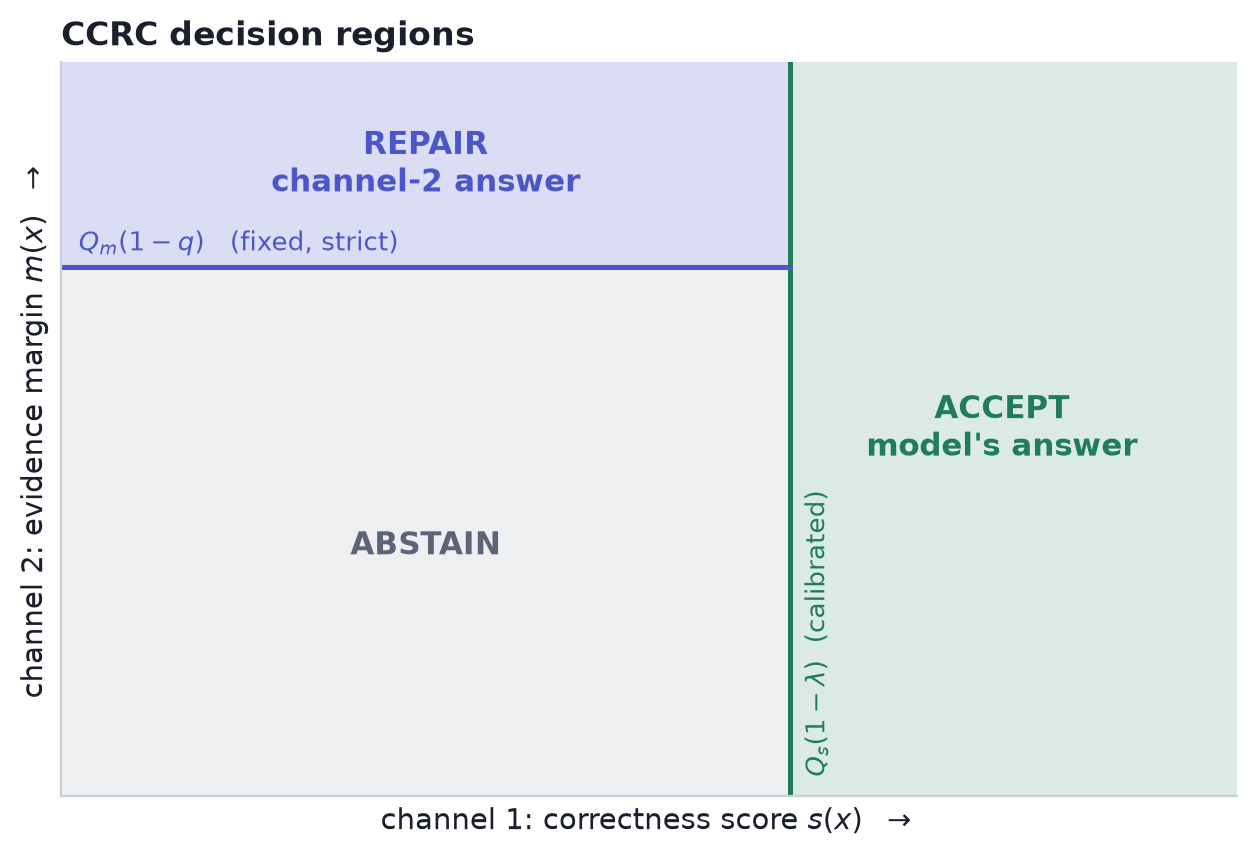
\includegraphics[width=0.62\textwidth]{fig_method.png}
\caption{CCRC partitions the $(s,m)$ plane. The acceptance threshold $Q_s(1-\lambda)$ is
calibrated; the repair gate $Q_m(1-q)$ is fixed in advance and strict, so that as $\lambda$
loosens the accepted region grows and the repair region shrinks. Keeping $q$ fixed is what
makes the family nested and lets a single fixed-sequence test suffice
(\S\ref{sec:decoupling}).}
\label{fig:method}
\end{figure}

\subsection{Worked examples on real data}
\label{sec:qualitative}

Before turning to aggregates, Figure~\ref{fig:qualitative} shows what the three decisions
look like on individual POPE images, with the actual channel-1 score, channel-2 detection
confidence, and resulting action for each. The three columns illustrate the regimes the
procedure is designed to separate.

In the \textsc{accept} column the model answers a straightforward existence question
confidently and correctly, the detector agrees, and the item is emitted unchanged; these
cases carry the bulk of the coverage. The \textsc{repair} column contains the cases that
motivate the method: LLaVA is asked whether a computer mouse is present, answers
``no'' with $p=0.21$, and is \emph{wrong} --- the mouse is there. Channel~1 correctly
assigns a low correctness score ($s=0.18$), which under a filtering policy would produce an
abstention and no answer at all. The detector, however, localises the object with confidence
$0.90$, comfortably inside the top evidence decile, so CCRC substitutes the detector's
answer and the item is emitted \emph{correctly}. This is the dilution effect of
\S\ref{sec:mechanism} in a single instance: a high-precision repair converts an item that
filtering would discard into a low-risk emitted item.

The \textsc{abstain} column shows the necessary complement. Here the model is wrong
\emph{and} the detector is also wrong, with weak evidence in both cases ($m=0.04$ and
$m=0.03$); the questions ask about a handbag and a truck that are not present, and neither
channel supplies a certifiable answer. Abstention is the correct action, and no amount of
substitution would help. The existence of a substantial population of such items is why
CCRC's gains are bounded by Proposition~\ref{prop:precondition} rather than being able to
recover the entire abstained mass.

\begin{figure}[t]
\centering
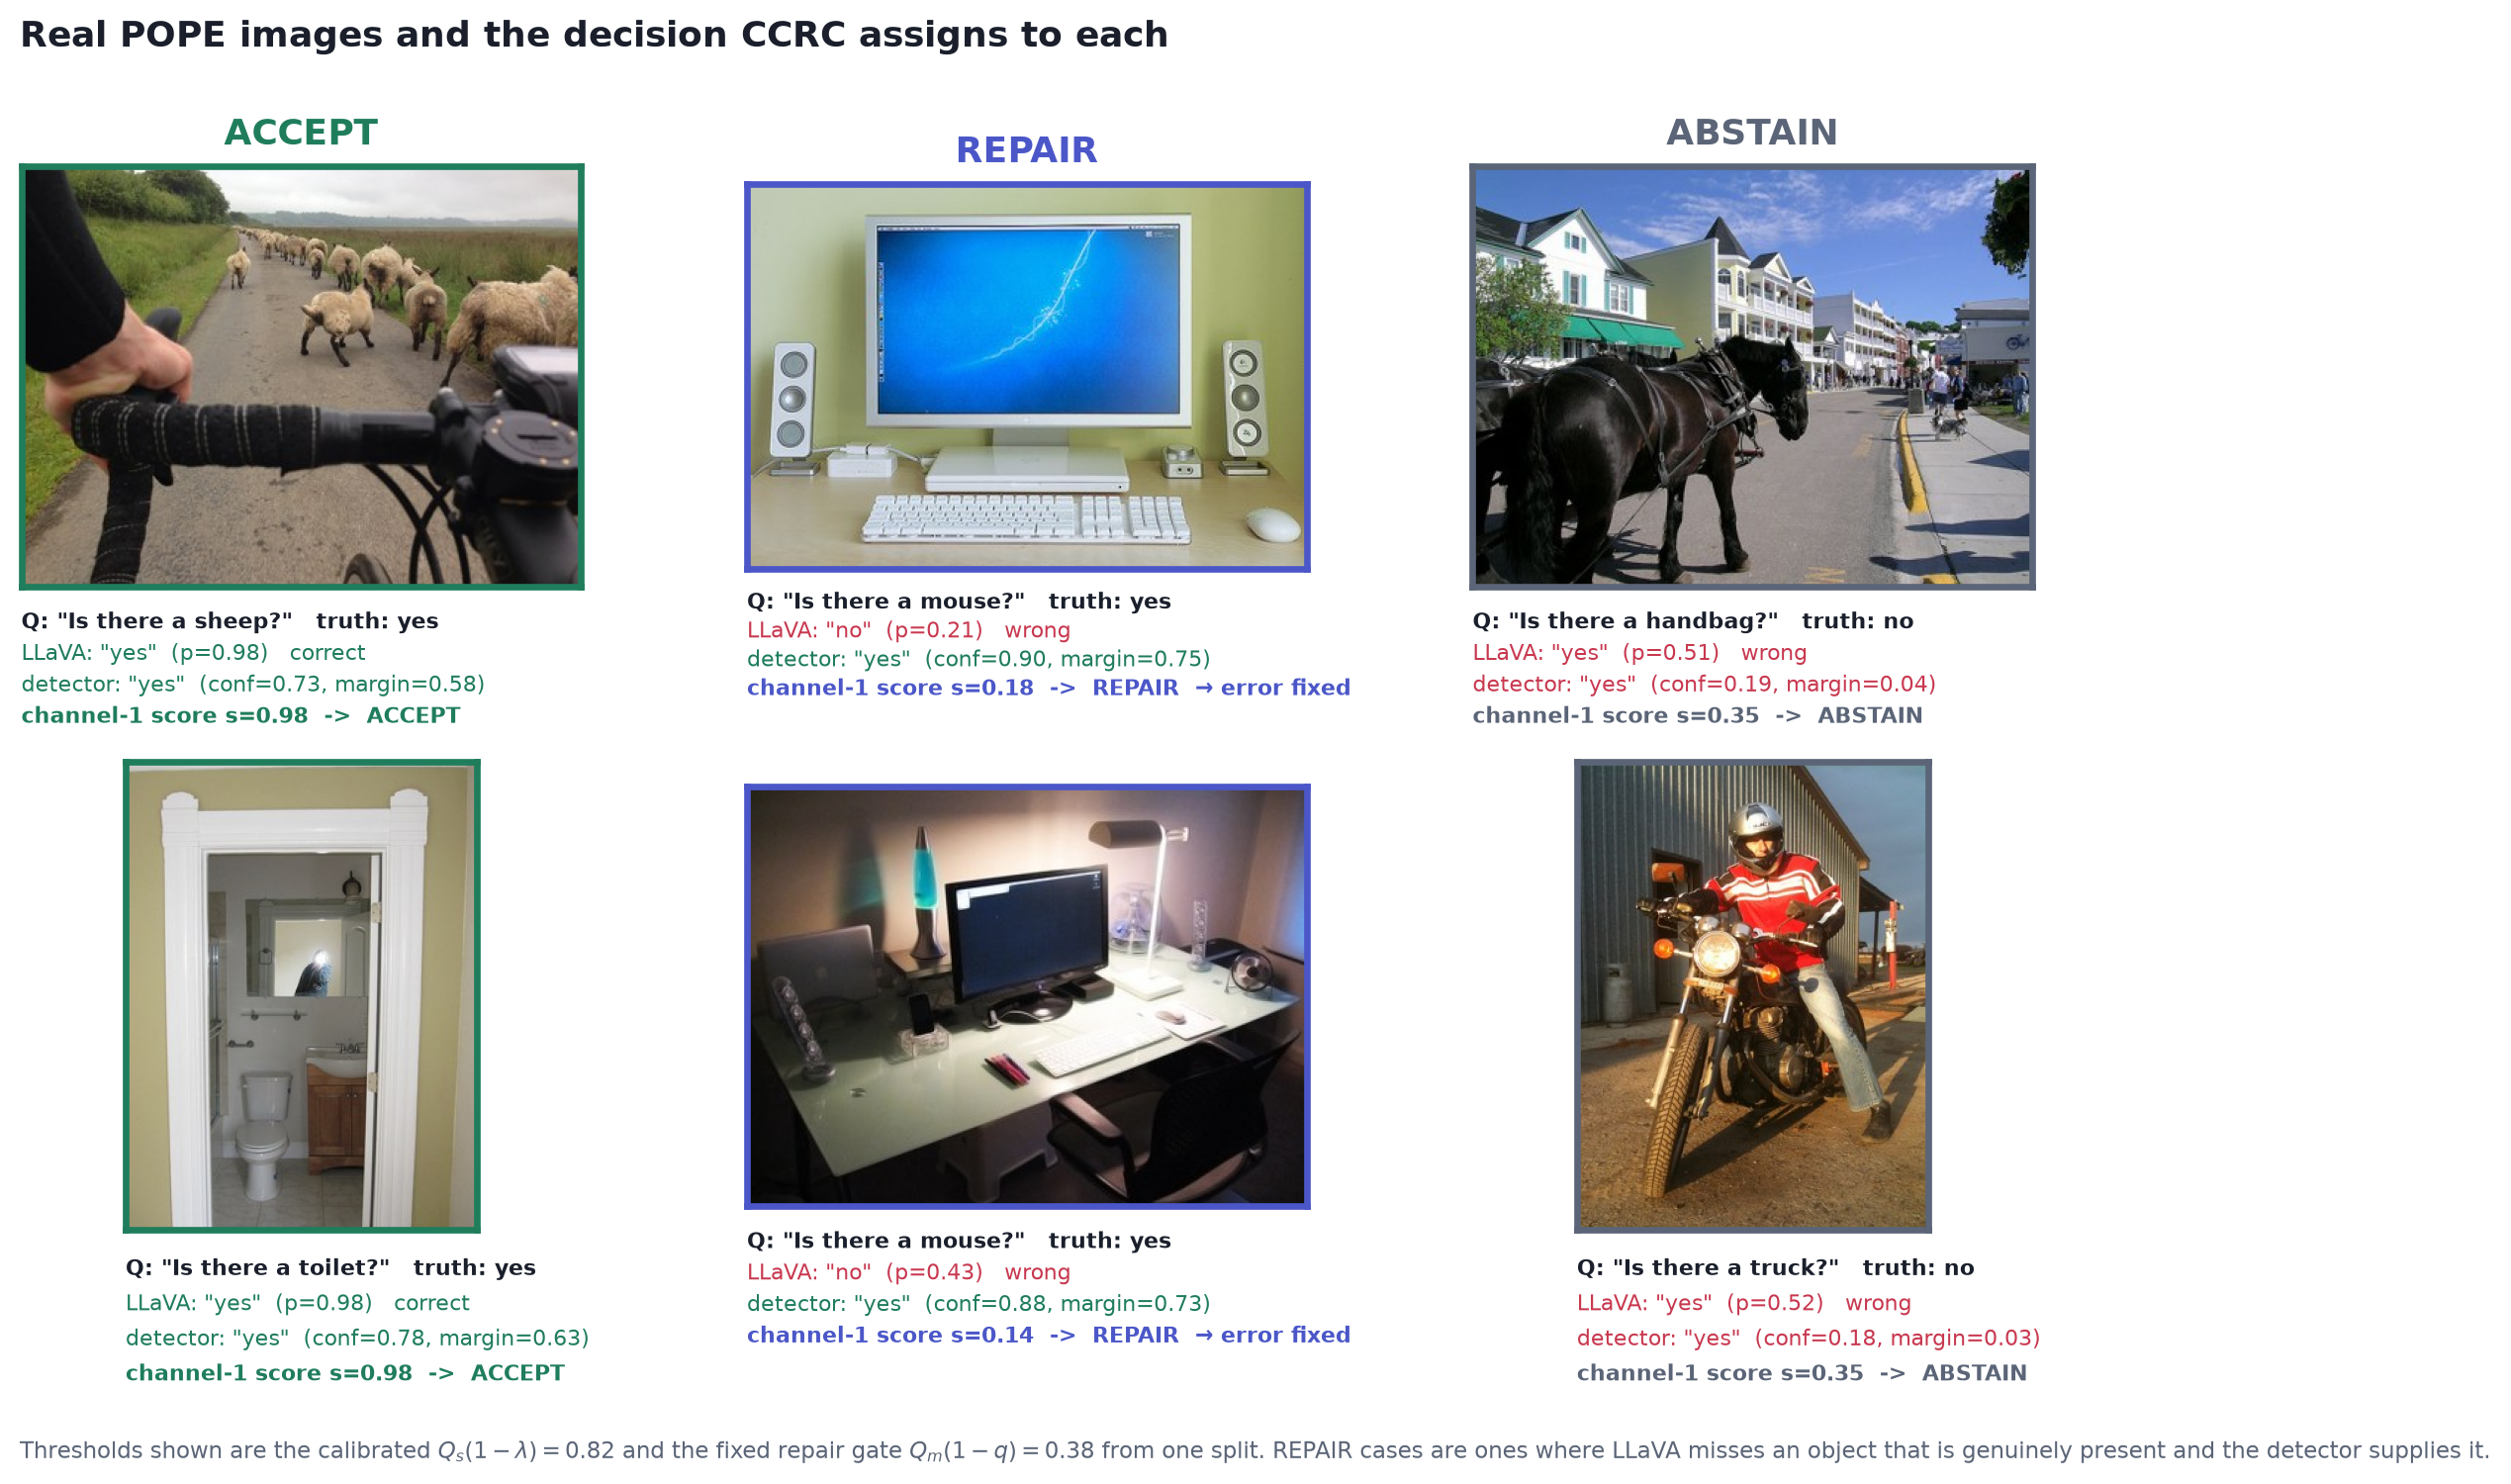
\includegraphics[width=\textwidth]{fig_qualitative.png}
\caption{Real POPE images with the actual quantities CCRC uses. Each panel reports the
question, the ground truth, LLaVA's answer with its probability, the detector's answer with
its confidence and evidence margin, the channel-1 correctness score, and the resulting
decision. \textbf{Accept} (left): both channels agree and the model is right.
\textbf{Repair} (centre): the model misses an object that is genuinely present and receives
a low correctness score, while the detector localises it with high confidence, so the
answer is substituted and the error is fixed --- items a filtering policy would abstain on.
\textbf{Abstain} (right): the model is wrong and the detector is also wrong with weak
evidence, so no certifiable answer exists and the procedure correctly declines. Thresholds
are the calibrated $Q_s(1-\lambda)$ and the fixed gate $Q_m(1-q)$ from one split.}
\label{fig:qualitative}
\end{figure}

\subsection{Validity}
\label{sec:validity}

\begin{theorem}[CCRC validity]
\label{thm:validity}
Let Assumptions~\ref{ass:exch}--\ref{ass:family} hold, let $\mathcal{T}=\{t_1>\dots>t_M\}$
and the repair gate $g$ be fixed before calibration, and let
\[
U(e,k;\delta)=\sup\{p:\Pr[\mathrm{Bin}(k,p)\le e]>\delta\}
\]
be the one-sided Clopper--Pearson upper confidence bound. Define
$\hat t$ by fixed-sequence testing: proceed through $j=1,2,\dots$ while
$U(V_{t_j},K_{t_j};\delta)\le\alpha$ on the calibration fold, and set
$\hat t$ to the last index that passed. Then the deployed policy
$\pi_{\hat t}$ satisfies
\[
\Pr\bigl[\Risk(\emit_{\hat t})\le\alpha\bigr]\ \ge\ 1-\delta .
\]
\end{theorem}

\begin{proof}
Fix $j$ and consider the null $H_j:\Risk(\emit_{t_j})>\alpha$. Because $t_j$ and $g$ are
constants, membership in the emitted set,
$\{s_i\ge t_j\}\cup\{s_i<t_j,\ m_i\ge g\}$, is a function of item $i$ alone, and each emitted
item contributes exactly one error indicator: $1-Y_i$ if accepted, $1-Y^{(2)}_i$ if repaired.
Under Assumption~\ref{ass:exch} the items are exchangeable draws, so conditional on
$K_{t_j}=k$ the $k$ emitted indicators are i.i.d.\ Bernoulli with common mean
$\Risk(\emit_{t_j})$ --- selection is by a set fixed in advance, which does not tilt the
conditional error probability, and $k$ is random but ancillary. Hence
$V_{t_j}\mid K_{t_j}=k\sim\mathrm{Bin}\bigl(k,\Risk(\emit_{t_j})\bigr)$ and, by construction of
the Clopper--Pearson bound, $\Pr[U(V_{t_j},k;\delta)\le\alpha\mid H_j]\le\delta$: the event
that the bound certifies a policy whose true risk exceeds $\alpha$ has probability at most
$\delta$, so $\phi_j=\mathbf{1}\{U\le\alpha\}$ is a valid level-$\delta$ test of $H_j$.

The index set and its ordering are pre-specified by Assumption~\ref{ass:family}, which is all
that fixed-sequence testing requires: testing $H_1,H_2,\dots$ in that order and stopping at
the first non-rejection controls the family-wise error rate at $\delta$ without any
multiplicity correction \citep{angelopoulos2021ltt}. The returned $\hat t$ is among the
rejected hypotheses, so with probability at least $1-\delta$ every rejected $H_j$ is false,
i.e.\ $\Risk(\emit_{\hat t})\le\alpha$.
\end{proof}

Two structural remarks follow; the second is the one a careful reader should hold us to.

\begin{remark}[why the mixture is not a complication, and why nesting is not a hypothesis]
The proof needs only that each emitted item contributes one $\{0,1\}$ error indicator and that
the set it is drawn from is fixed in advance. Whether that indicator refers to the model's
answer or to channel~2's is irrelevant, which is precisely why Proposition~\ref{prop:floor}
does not bind: its premise restricts the \emph{action space}, which the guarantee itself never
uses. Nesting is likewise not a validity hypothesis, but it is what makes the procedure
powerful: because $g$ is fixed, $A_t$ grows and $R_t$ shrinks as $t$ falls, so
$\emit_t=A_t\cup M$ with $M=\{m\ge g\}$ constant, and \emph{coverage} increases along the grid
even though the risk need not --- which is what makes ``the last index that passed'' the right
thing to return.
\end{remark}

\begin{remark}[value-indexed versus rank-indexed families]
\label{rem:rankvsvalue}
The natural alternative indexes the family by quantiles, $t=Q_s(1-\lambda)$ with
$Q_s$ the empirical quantile of the \emph{same} calibration fold whose errors are counted, and
would like the emitted-error count to be binomial with mean $k\,\Risk$. That step is where the
difficulty actually lives, and it does not hold: selecting the top
$\lceil\lambda n_{\mathrm{cal}}\rceil$ items by score makes $k$ deterministic and makes the
selection event a function of all items jointly, so conditionally on the calibration features
the emitted indicators have item-specific means and $V$ is \emph{Poisson binomial} rather than
binomial. Poisson-binomial lower tails are dominated by the equal-mean binomial
\citep{hoeffding1956}, which points in the conservative direction, but that domination is not
by itself a treatment of the order-statistic selection effect. Indexing by score \emph{values}
removes the problem instead of bounding it, at the price of one extra pre-specification, and
it costs nothing in practice: a value grid may be laid down on a held-out score histogram, as
Algorithm~\ref{alg:ccrc} does.

We nonetheless report measurements from the rank-indexed implementation throughout, because it
is what our scripts run and what a practitioner without a pre-specified value grid would write.
Two pieces of evidence bound the exposure. First, a synthetic study in which the population risk
of the selected policy is known exactly: over four score shapes (well-separated logistic, weakly
separated, heavy-tailed, and a miscalibrated monotone transform) $\times$ four calibration sizes
($100$, $250$, $500$, $1500$), the realised exceedance $\Pr[\Risk(\emit_{\hat\lambda})>\alpha]$
of the rank-indexed procedure is $0.0$--$5.9\%$ against $\delta=0.10$ --- conservative in all
sixteen cells, and nowhere near the nominal level. Second, on real data the population-risk
exceedance is $0.0$--$5.1\%$ across all $40$ cells of \S\ref{sec:exp}
(Table~\ref{tab:audit}). We therefore claim the theorem for the value-indexed family, and for
the rank-indexed variant we claim empirical validity with a stated margin, not a proof.

One methodological note on that simulation, because it bears on how the audit tables in this
paper should be read. The guarantee is unconditional, and an aborted run emits nothing and so
cannot violate it; the $0.0$--$5.9\%$ above therefore counts aborted draws as compliant.
Conditional on the procedure certifying \emph{something}, exceedance in the same simulation
reaches much higher values on the cells where aborts dominate --- up to $100\%$ in a cell whose
abort rate is also $100\%$, which is a statement about a handful of lucky draws and not about
validity. Our real-data audit uses the conditional convention (Table~\ref{tab:audit} excludes
aborted splits and prints the abort rate beside each figure), which is the conservative choice;
it stays below $\delta$ everywhere on real data only because the real abort rates in that table
are small.
\end{remark}

\begin{lemma}[Minimum certifiable emitted-set size]
\label{lem:kmin}
With zero observed errors, $U(0,k;\delta)=1-\delta^{1/k}$. Hence no emitted set of size
$k$ can be certified at level $\alpha$ unless
\[
k\ \ge\ k_{\min}=\frac{\ln\delta}{\ln(1-\alpha)} .
\]
For $\alpha=\delta=0.10$, $k_{\min}=\lceil 21.85\rceil=22$.
\end{lemma}

\begin{proof}
$\Pr[\mathrm{Bin}(k,p)\le 0]=(1-p)^k$, so the upper bound with $e=0$ solves
$(1-p)^k=\delta$, giving $U(0,k;\delta)=1-\delta^{1/k}$. This is decreasing in $k$, and
$1-\delta^{1/k}\le\alpha\iff\delta^{1/k}\ge1-\alpha\iff k^{-1}\ln\delta\ge\ln(1-\alpha)$;
dividing by the negative quantity $\ln(1-\alpha)$ reverses the inequality and yields
$k\ge\ln\delta/\ln(1-\alpha)$. Since $U(e,k;\delta)\ge U(0,k;\delta)$ for $e\ge0$, no error
count can do better.
\end{proof}

Lemma~\ref{lem:kmin} is elementary but consequential: a fixed sequence whose first policy
emits fewer than $k_{\min}$ items fails at step one and, because fixed-sequence testing
stops at the first non-rejection, returns \emph{zero} coverage. We encountered exactly this
failure and now begin the grid at the analytically derived minimum. It turns out to be the
single most consequential fact in the paper's empirical half: \S\ref{sec:kminfail} shows that
the same mechanism, one step further on, explains a weak score certifying nothing rather than
less, the collapse of self-repair, and our one negative result.

\subsection{Why repairs cannot be self-certified in practice}
\label{sec:independence}

The most economical design would avoid a second channel: if $s$ says the model is probably
wrong, emit the opposite. This section shows why that fails. The argument has to be made at
the level of the \emph{mixture}, because that is what CCRC certifies --- a repair region
whose own risk exceeds $\alpha$ is not automatically inadmissible, since a compliant blend
can absorb it (Proposition~\ref{prop:dilution}). The correct statement is therefore not
that self-repair is impossible but that it is \emph{self-defeating}: the mass it can buy is
bounded by the accepted region's slack, and the fixed-sequence test aborts before it can be
collected.

\begin{proposition}[Self-repair is bounded by slack, and is not free]
\label{prop:selfrepair}
Suppose the answer space is binary and the repair is the negation of the model's answer, so
that $Y^{(2)}=1-Y$. Let $R\subseteq\mathcal{X}$ be any repair region with mass $c_r$ and let
the accepted region have mass $c_a$ and risk $r_a$. Then the risk of the repaired region is
\[
  r_r \;=\; \Pr[\text{repaired answer wrong}\mid X\in R] \;=\; \Pr[Y=1\mid X\in R],
\]
i.e.\ exactly the model's \textbf{accuracy} on $R$. Consequently, if $r_r>\alpha$ the
mixture is compliant only for
\begin{equation}
\label{eq:selfrepair}
  c_r \;\le\; c_a\,\frac{\alpha-r_a}{r_r-\alpha},
\end{equation}
and a region of accuracy $\le\alpha$ --- for which no such constraint binds --- requires the
score to isolate inputs on which the model is right less than $\alpha$ of the time. That is
strictly stronger than isolating inputs of low \emph{confidence}, and no monotone
transformation of $s$ can supply the difference.
\end{proposition}

\begin{proof}
On $R$ the emitted answer is $1-\hat a$, which is correct exactly when $\hat a$ is
incorrect; its error indicator is therefore $Y$, and averaging over $R$ gives
$r_r=\Pr[Y=1\mid X\in R]$. For the mixture,
$\bar r=(c_ar_a+c_rr_r)/(c_a+c_r)\le\alpha$ rearranges to
$c_r(r_r-\alpha)\le c_a(\alpha-r_a)$, which is \eqref{eq:selfrepair} when $r_r>\alpha$ and
is vacuous when $r_r\le\alpha$. The final claim follows because any repair rule of the form
$\{s(X)\le t\}$ has $r_r=\Pr[Y=1\mid s(X)\le t]$, a functional of the joint law of $(s,Y)$
invariant to monotone reparameterisation of $s$.
\end{proof}

Proposition~\ref{prop:selfrepair} converts an intuition --- ``a hallucination score reports
suspicion, not knowledge of the truth'' --- into a budget. Two measurements show how little
that budget buys.

\paragraph{No low-accuracy region exists where it is needed.}
The model's accuracy in the bottom $2\%$ of $s$ --- which is exactly $r_r$, the flip region's
own risk --- is $22.1\%$ on POPE-1500 and $43.8\%$ on POPE-adversarial against $\alpha=0.10$;
in the bottom decile it is $42.8\%$ and $47.3\%$. On Qwen2-VL the bottom $2\%$ is \emph{above}
chance at $62.4\%$, so flipping there is actively harmful. Only two settings contain a flippable
region at all, VCD-decoded LLaVA at $4.9\%$ and AMBER at $0.9\%$, and they are the two settings
whose \emph{accepted region has the least slack to spend}: AMBER already certifies $91.8\%$ of
its inputs at $\alpha=0.10$ and VCD's accepted risk sits close to the budget. (This is a
statement about slack in \eqref{eq:selfrepair}, not about headroom $\mu-\alpha$: VCD in fact has
the \emph{largest} headroom of our five settings, $9.6$ points, and AMBER the smallest, $1.4$;
the two quantities are easy to conflate and point in opposite directions here.)

\paragraph{The fixed sequence aborts before the slack can be spent.}
Substituting the negation of the model's answer at $q=0.02$ and certifying the mixture exactly
as in \S\ref{sec:validity}, certified coverage falls by $49.3$, $37.3$, $76.9$ and $6.6$ points
on the four POPE settings at $\alpha=0.10$ (all $p<10^{-7}$; Table~\ref{tab:selfrepair}). The
mechanism is not a graceful trade: the fixed sequence returns \emph{nothing at all} on
$73.0\%$, $88.8\%$, $98.8\%$ and $25.2\%$ of splits respectively. The reason is structural. The
self-repair region has fixed mass, so at the \emph{start} of the grid --- where the accepted set
is smallest and $K$ barely clears $k_{\min}$ --- it is the largest fraction of the emitted set
it will ever be, and its $4.9$--$62.4\%$ error rate fails the very first hypothesis.
Fixed-sequence testing must stop at the first non-rejection (\S\ref{sec:validity}), so the
procedure never reaches the later thresholds at which \eqref{eq:selfrepair} would in fact be
satisfiable. Self-repair is defeated by the interaction between a fixed-mass, high-error repair
block and the prefix structure of the test, not by the region being uncertifiable in isolation.
This is the first of the three instances of that interaction collected in
\S\ref{sec:kminfail}.

\begin{table}[t]
\centering
\caption{Self-certified repair: flipping the model's answer on the bottom $q=0.02$ of $s$ and
certifying the mixture, against filtering, under the identical protocol ($400$ paired splits,
$\delta=0.10$). $r_r$ is the flip region's own risk, i.e.\ the model's accuracy there. All
$p$-values are two-sided paired $t$-tests on the $400$ paired differences. The gain is
negative wherever the abort rate is large, and positive only where $r_r$ is small.}
\label{tab:selfrepair}
\small
\resizebox{\textwidth}{!}{%
\begin{tabular}{lcccccc}
\toprule
Setting ($\alpha=0.10$) & $r_r$ & Filter & Self-repair & Gain [95\% CI] & $p$ & abort\\
\midrule
POPE-1500 LLaVA    & 22.1\% & 68.6\% & 19.3\% & $-49.3$ $[-52.5,-46.1]$ & $4\!\times\!10^{-106}$ & 73.0\%\\
POPE-adv LLaVA     & 43.8\% & 44.0\% & \phantom{0}6.6\% & $-37.3$ $[-40.1,-34.5]$ & $2\!\times\!10^{-88}$ & 88.8\%\\
POPE-adv Qwen2-VL  & 62.4\% & 77.9\% & \phantom{0}1.1\% & $-76.9$ $[-78.6,-75.1]$ & $1\!\times\!10^{-261}$ & 98.8\%\\
POPE-adv LLaVA+VCD & \phantom{0}4.9\% & 48.8\% & 42.2\% & $-6.6$ $[-8.9,-4.3]$ & $4\!\times\!10^{-8}$ & 25.2\%\\
AMBER(d) LLaVA     & \phantom{0}0.9\% & 91.8\% & 92.7\% & $+0.9$ $[-0.6,+2.5]$ & $0.25$ (n.s.) & \phantom{0}2.8\%\\
\midrule
\multicolumn{7}{l}{\emph{at $\alpha=0.15$, the two clean-flip-region cells become positive:}}\\
POPE-adv LLaVA+VCD & \phantom{0}4.9\% & 75.8\% & 77.7\% & $+1.9$ $[+0.6,+3.3]$ & $0.006$ & \phantom{0}2.5\%\\
AMBER(d) LLaVA     & \phantom{0}0.9\% & 95.9\% & 98.7\% & $+2.9$ $[+2.6,+3.1]$ & $6\!\times\!10^{-78}$ & \phantom{0}0.0\%\\
\bottomrule
\end{tabular}
}
\end{table}

\paragraph{What this licenses us to claim.}
Not that certified correction is impossible without a second channel. Equation
\eqref{eq:selfrepair} admits self-repair whenever the accepted region has slack and the flip
region is clean enough, and that is confirmed rather than refuted by the two cells where both
conditions hold: at $\alpha=0.15$ self-repair gains $+2.9$ points on AMBER
($p=6\times10^{-78}$) and $+1.9$ on VCD ($p=0.006$). At $\alpha=0.10$ the AMBER cell is
$+0.9$ points with $95\%$ CI $[-0.6,+2.5]$, $p=0.25$: not distinguishable from zero, and we do
not count it. What the measurements license is the weaker and sufficient claim that \emph{on the
settings where filtering is expensive enough for correction to be worth doing, no
self-certifiable flip region exists}, so a second channel is required in practice. We state this
as an empirical regularity with a mechanism, not as a theorem, and \S\ref{sec:discussion} lists
it among the claims most likely to fail on a new benchmark.

Channel 2 escapes the budget in \eqref{eq:selfrepair} because $Y^{(2)}$ is a genuinely
different random variable, not a deterministic function of $Y$. The top evidence decile, which
is the only decile repairs are drawn from, is $100\%$ accurate on POPE
(Table~\ref{tab:channel2}), so $r_r$ there is far below $\alpha$ and the constraint is vacuous
rather than binding.

\begin{table}[t]
\centering
\caption{Channel-2 (detector) accuracy by evidence-margin decile on POPE-1500 ($150$ items per
decile). Repairs are drawn only from the top decile, where accuracy is $100\%$, far above
$1-\alpha$. Accuracy improves with the margin but not monotonically --- the 5th falls below the
4th and the 8th below the 7th --- which is why the repair gate must be strict rather than merely
above the median. All ten deciles are printed because the non-monotonicity is the point.}
\label{tab:channel2}
\small
\resizebox{\textwidth}{!}{%
\begin{tabular}{lcccccccccc}
\toprule
Margin decile & 1 (bottom) & 2 & 3 & 4 & 5 & 6 & 7 & 8 & 9 & 10 (top)\\
\midrule
Detector accuracy & 0.513 & 0.713 & 0.733 & 0.807 & 0.772 & 0.934 & 0.953 & 0.927 & 0.960 & 1.000\\
\bottomrule
\end{tabular}
}
\end{table}

\subsection{Why the repair gate must be decoupled}
\label{sec:decoupling}

The obvious first version of the procedure ties the repair gate to $\lambda$, i.e.\ uses
$m(x)\ge Q_m(1-\lambda)$ in \eqref{eq:policy}. This is natural but harmful: as $\lambda$
loosens to admit more accepted items, the repair gate loosens in step and begins admitting
low-precision repairs, so the fixed sequence terminates earlier. Empirically the coupled
version gained on LLaVA ($+4.7$, $+5.3$ points) but \emph{lost} on Qwen2-VL ($-4.2$) and on
a VCD-decoded model ($-2.9$). It also required certifying two families (with and without
repair) at $\delta/2$ and selecting between them, wasting half the confidence budget.

Fixing $q$ removes both problems. The family becomes nested in the single threshold
$t$, so one fixed-sequence test at full $\delta$ suffices (Theorem~\ref{thm:validity}), and
repair precision is held constant while $t$ sweeps. Table~\ref{tab:qsens} reports the
sensitivity over all ten cells.

\begin{table}[t]
\centering
\caption{Sensitivity to the repair gate $q$: change in certified coverage relative to
filtering, over five settings $\times$ two risk levels ($400$ paired splits). Bracketed
figures are $95\%$ CIs on the mean paired gain. The two negative cells at $q=0.10$ are the two
AMBER cells; restricting the table to the eight POPE cells would exclude the loss, so all ten
are shown.}
\label{tab:qsens}
\small
\resizebox{\textwidth}{!}{%
\begin{tabular}{lcccc}
\toprule
Setting & $\alpha$ & $q=0.10$ & $q=0.25$ & $q=0.50$\\
\midrule
POPE-1500 LLaVA    & 0.10 & $+3.18$ $[+2.6,+3.8]$  & $+5.39$ $[+3.9,+6.9]$   & $+8.84$ $[+7.7,+10.0]$\\
POPE-adv LLaVA     & 0.10 & $+3.19$ $[+1.7,+4.7]$  & $-0.05$ $[-2.9,+2.8]$   & $+2.04$ $[-1.4,+5.5]$\\
POPE-adv Qwen2-VL  & 0.10 & $+1.60$ $[+0.8,+2.4]$  & $-16.44$ $[-20.0,-12.9]$& $-14.86$ $[-18.3,-11.4]$\\
POPE-adv LLaVA+VCD & 0.10 & $+2.15$ $[+1.3,+3.0]$  & $-6.35$ $[-9.2,-3.5]$   & $-9.04$ $[-12.0,-6.1]$\\
AMBER(d) LLaVA     & 0.10 & $-10.20$ $[-13.4,-7.0]$& $-38.69$ $[-43.3,-34.1]$& $-25.91$ $[-30.2,-21.6]$\\
\midrule
POPE-1500 LLaVA    & 0.15 & $+1.95$ $[+1.8,+2.1]$  & $+5.38$ $[+5.2,+5.6]$   & $+6.78$ $[+6.6,+7.0]$\\
POPE-adv LLaVA     & 0.15 & $+7.59$ $[+5.5,+9.7]$  & $+10.14$ $[+7.7,+12.6]$ & $+14.47$ $[+12.0,+16.9]$\\
POPE-adv Qwen2-VL  & 0.15 & $+0.40$ $[+0.3,+0.5]$  & $-1.22$ $[-2.6,+0.2]$   & $+0.28$ $[-0.7,+1.3]$\\
POPE-adv LLaVA+VCD & 0.15 & $+1.39$ $[+0.5,+2.3]$  & $+0.48$ $[-1.0,+2.0]$   & $+1.40$ $[+0.1,+2.7]$\\
AMBER(d) LLaVA     & 0.15 & $-11.90$ $[-15.1,-8.7]$& $-11.55$ $[-14.7,-8.4]$ & $-2.19$ $[-3.8,-0.6]$\\
\midrule
\textbf{cells positive} & & \textbf{8 / 10} & 5 / 10 & 6 / 10\\
\textbf{range}          & & $-11.90$ to $+7.59$ & $-38.69$ to $+10.14$ & $-25.91$ to $+14.47$\\
\textbf{worst abort rate}& & 17.5\% & 43.8\% & 36.0\%\\
\bottomrule
\end{tabular}
}
\end{table}

\subsection{What ``$q$ is fixed a priori'' can and cannot mean}
\label{sec:qsel}
Asserting that $q$ is fixed in advance and not tuned would not be defensible next to a table
showing $q=0.10$ to be the best of three values on the same cells that produce the headline.
Table~\ref{tab:qsens} makes the honest version available. Three statements, in decreasing order
of comfort.

First, \textbf{$q=0.10$ is not the best value by gain.} At $\alpha=0.15$, $q=0.50$ wins all
five cells, and it also wins POPE-1500 at $\alpha=0.10$; the mean gain over the eight POPE
cells is $+2.66$ at $q=0.10$ against $+4.89$ for a per-cell oracle. What $q=0.10$ is best at is
\emph{robustness}: it is positive in $8$ of $10$ cells against $5$ and $6$, its worst cell is
three times less bad, and its worst abort rate is less than half. That is a legitimate reason
to prefer a strict gate and it is the reason we do.

Second, \textbf{the selection exposure is small and points the wrong way for us.} Choosing $q$
by leave-one-dataset-out --- maximising mean gain on the other datasets at the deployment
$\alpha$, which is user-specified rather than tuned --- yields a mean gain of $+4.19$ points over
the eight POPE cells against the $+2.66$ we report for fixed $q=0.10$, with an oracle--LODO gap
(the actual selection exposure) of $+0.70$ points. A properly transferred choice of $q$ would
therefore make this paper's numbers \emph{larger}; the reported configuration is conservative.

Third, \textbf{$q$ must be indexed to $\alpha$.} Conditional on $\alpha$, the LODO choice is
stable ($q=0.10$ at $\alpha=0.10$, $q=0.50$ at $\alpha=0.15$, on every fold). Pooling across
$\alpha$ destroys it: the pooled rule picks $q=0.50$ for the Qwen $\alpha=0.10$ fold and turns
$+1.31$ into $-14.71$. Anyone transporting our recommendation to a different risk target should
re-select, not reuse. Appendix~\ref{app:qdelta} reports a fully valid alternative that removes
the objection outright --- certify all three $q$ at $\delta/3$ and select on the calibration fold
--- at a mean cost of $+0.50$ points relative to the reported configuration.

\subsection{Why it gains: dilution, and how much of the gain it explains}
\label{sec:mechanism}

Our initial hypothesis was that repairs \emph{spend} the accepted set's unused risk budget:
filtering typically realises a risk below $\alpha$ (we measure $8.0\%$ at $\alpha=0.10$),
and repairs with error above $\alpha$ could be admitted while the blend stayed compliant.
The measured effect runs the other way, and is stronger.

\begin{proposition}[Dilution lowers the emitted risk pointwise in $\lambda$]
\label{prop:dilution}
Fix $\lambda$ and let the accepted set have mass $c_a$ and risk $r_a$, and the repair set
mass $c_r$ and risk $r_r$. The emitted risk is the mixture
$\bar r=(c_ar_a+c_rr_r)/(c_a+c_r)$. If $r_r<r_a$ then $\bar r<r_a$, strictly decreasing in
$c_r$, so every $\lambda$ that is population-feasible for filtering remains
population-feasible with repairs and further $\lambda$ may become feasible. If instead
$r_r>\alpha>r_a$, admitting repairs consumes slack and may render feasible $\lambda$
infeasible.
\end{proposition}

\begin{proof}
$\bar r-r_a=c_r(r_r-r_a)/(c_a+c_r)$, which is negative iff $r_r<r_a$, and
$\partial\bar r/\partial c_r=c_a(r_r-r_a)/(c_a+c_r)^2$ has the same sign. Filtering is the
special case $c_r=0$, giving the feasibility claim. The last statement is the same
computation with the inequality reversed.
\end{proof}

\begin{remark}[Why this does not immediately imply a more permissive $\hat\lambda$]
\label{rem:prefix}
Proposition~\ref{prop:dilution} is a statement about the \emph{population} risk at fixed
$\lambda$, and two gaps separate it from the certified $\hat\lambda$ the procedure returns.
First, $\hat\lambda$ is chosen by a Clopper--Pearson bound on realised counts, not by
population feasibility: a single repaired item that happens to be wrong raises $V_\lambda$
and can tighten $\hat\lambda$ even when $r_r<r_a$. Second, fixed-sequence testing stops at
the first non-rejection, so a larger feasible \emph{set} yields a later stopping index only
if feasibility is a \emph{prefix} of the grid --- which is risk monotonicity in $\lambda$,
exactly what \S\ref{sec:validity} declines to assume. We therefore treat the coverage gain
as an empirical claim (\S\ref{sec:ccrcresults}) for which Proposition~\ref{prop:dilution}
supplies the mechanism, not a corollary. \S\ref{sec:independence} exhibits the failure mode
this remark anticipates: there, feasibility is not a prefix and the test aborts at the first
index.
\end{remark}

The empirically relevant regime is the first. Because repairs are drawn from the top
evidence decile, their risk is \emph{lower} than that of the acceptance gate's
\emph{marginal} items --- the items that determine whether the constraint binds. Repairs
therefore act as ballast: a small high-precision mass pulls $\bar r$ down and can let the
threshold open further.

\paragraph{How much of the gain is that, and how much is arithmetic.}
One tempting way to report the effect is a ``leverage multiplier'': the small repaired mass
buying more coverage than its own size. That framing is largely tautological and we do
not use it. Repaired items are \emph{themselves emitted}, so whenever
$\hat\lambda$ does not fall, CCRC emits exactly filtering's accepted set plus the gated repairs
and the gain is mechanically equal to the repaired mass --- no dilution required, and nothing
about the mechanism demonstrated. The quantity that does demonstrate it is the \emph{extra
accepted} mass admitted because $\hat\lambda$ actually moved. So we decompose the gain per
split into
\[
\underbrace{\text{repairs available at filtering's own }\hat\lambda}_{\text{(i) automatic}}
\;+\;\underbrace{\text{everything else}}_{\text{(ii) dilution}},
\]
computed on the splits where both arms certify something, and report both
(Table~\ref{tab:dilution}).

Two facts govern the reading. $\hat\lambda$ is \emph{identical} between filtering and CCRC on
$70.6$--$87.7\%$ of splits at $\alpha=0.10$ and $76.5$--$98.3\%$ at $\alpha=0.15$; on those
splits there is no dilution effect at all, by construction. And where it does move, the payoff
is real but small: term (ii) is $+0.20$ to $+1.84$ points at $\alpha=0.10$ and $+0.00$ to
$+0.65$ at $\alpha=0.15$, and it is not distinguishable from zero on two cells (POPE-adv LLaVA
at $\alpha=0.15$, $p=0.41$; AMBER at $\alpha=0.15$, $p=0.32$). Term (iii) in the table, the
mass \emph{lost} from the repair set as $\lambda$ opens and absorbs it, is small and negative
everywhere, which is the nesting the method assumes showing up in the data.

\begin{table}[t]
\centering
\caption{Decomposition of the CCRC gain at $\alpha=0.10$ into the part that is automatic and the
part attributable to dilution ($400$ paired splits, conditioned on both arms certifying;
abort rates are reported separately in Table~\ref{tab:ccrc}). Term (i) is the repaired mass
available at filtering's own threshold, which is emitted whether or not the threshold moves;
term (ii) is the extra accepted mass admitted because it did. ``$\hat\lambda$ moves'' is the
fraction of splits on which the two arms select different thresholds. $p$-values are two-sided
paired $t$-tests on term (ii).}
\label{tab:dilution}
\small
\resizebox{\textwidth}{!}{%
\begin{tabular}{lccccc}
\toprule
Setting & $\hat\lambda$ moves & gain & (i) repairs emitted & (ii) dilution [95\% CI] & $p$(ii)\\
\midrule
POPE-1500 LLaVA    & 28.0\% & $+2.68$ & $+1.82$ & $+0.86$ $[+0.63,+1.09]$ & $2\!\times\!10^{-12}$\\
POPE-adv LLaVA     & 29.4\% & $+3.59$ & $+1.74$ & $+1.84$ $[+1.22,+2.46]$ & $1\!\times\!10^{-8}$\\
POPE-adv Qwen2-VL  & 19.9\% & $+2.03$ & $+1.02$ & $+1.01$ $[+0.43,+1.59]$ & $7\!\times\!10^{-4}$\\
POPE-adv LLaVA+VCD & 12.3\% & $+2.05$ & $+0.97$ & $+1.08$ $[+0.62,+1.53]$ & $4\!\times\!10^{-6}$\\
AMBER(d) LLaVA     & 15.2\% & $+2.17$ & $+1.97$ & $+0.20$ $[+0.08,+0.31]$ & $9\!\times\!10^{-4}$\\
\midrule
\multicolumn{6}{l}{term (iii), repair mass absorbed as $\lambda$ opens: $-0.02$, $-0.05$,
$-0.03$, $-0.17$, $-0.17$ points respectively}\\
\bottomrule
\end{tabular}
}
\end{table}

The honest headline is therefore not leverage but cheapness: a small mass of near-certain
repairs can be added to the emitted set at essentially no risk cost, and \emph{on top of that}
dilution contributes a fraction of a point to $1.8$ points on the minority of splits where the
constraint actually loosens. Figure~\ref{fig:precondition}B plots the two terms. Note that the
AMBER row of Table~\ref{tab:dilution} is positive: conditional on certifying, AMBER behaves like
the other settings, which is the first sign that its reported loss is about something else
entirely (\S\ref{sec:kminfail}).

\subsection{When it helps: a checkable precondition}
\label{sec:precondition}

CCRC is not a free improvement. Its upside is bounded by what filtering leaves on the
table, while its downside --- perturbing a nearly-saturated constraint --- is not
symmetrically bounded.

\begin{proposition}[Gain is capped by abstained mass]
\label{prop:precondition}
Let $\Cov_{\mathrm{filt}}$ be the coverage certified by filtering at level $(\alpha,\delta)$
and $\Cov_{\mathrm{CCRC}}$ that certified by CCRC. Then
\[
\Cov_{\mathrm{CCRC}}-\Cov_{\mathrm{filt}}\ \le\ 1-\Cov_{\mathrm{filt}},
\]
and $1-\Cov_{\mathrm{filt}}\ge(\mu-\alpha)/(1-\alpha)$ by
Proposition~\ref{prop:floor}. No matching lower bound on $\Cov_{\mathrm{CCRC}}$ holds, so
the upside is bounded by the abstained mass while the downside is not.
\end{proposition}

\begin{proof}
Coverage is at most one, so the gain cannot exceed the abstained fraction
$1-\Cov_{\mathrm{filt}}$; the floor inequality is Proposition~\ref{prop:floor} applied to
the filtering policy. The asymmetry claim follows because
Proposition~\ref{prop:dilution} shows the emitted risk strictly increases when repairs are
admitted with $r_r>r_a$, and Remark~\ref{rem:prefix} shows this can move $\hat\lambda$
downward without bound.
\end{proof}

\begin{remark}[Why this is a diagnostic and not a prediction]
\label{rem:notprediction}
An upper bound on the gain cannot predict a loss. Write
$1-\Cov_{\mathrm{filt}}=(\mu-\alpha)/(1-\alpha)+\varepsilon$. One might hope $\varepsilon$
is small so that headroom $\mu-\alpha$ alone governs the achievable gain, but our own data
refutes it: on AMBER the floor is $1.6\%$ while $1-\Cov_{\mathrm{filt}}=8.2\%$, so
$\varepsilon=6.6\%$, four times the floor. The usable statement is therefore the crude one:
the gain cannot exceed the abstained mass, so a setting that already certifies most of its
inputs has little to win and the same exposure to loss.
\end{remark}

\paragraph{The headroom diagnostic, demoted.}
It is tempting to go further and read Proposition~\ref{prop:precondition} as \emph{predicting}
our one negative result, with AMBER --- $\mu=11.4\%$ against $\alpha=0.10$, floor $1.6\%$,
filtering already certifying $91.8\%$ --- as the confirming instance. That reading
does not survive \S\ref{sec:kminfail}, which shows AMBER's loss is an abort phenomenon and that
conditional on certifying anything CCRC \emph{wins} there. We therefore separate the proved
bound from the unproved diagnostic and label the latter honestly:

\begin{conjecture}[Headroom precondition; \emph{no confirming instance}]
\label{conj:headroom}
There is a threshold $h>0$ such that CCRC's certified-coverage gain over filtering is
non-negative whenever the headroom $\mu-\alpha$ exceeds $h$ and an applicable evidence channel
exists, and that settings with $\mu-\alpha<h$ are at material risk of a loss.
\end{conjecture}

We state this as a conjecture because we have no evidence for it. The bound of
Proposition~\ref{prop:precondition} is true but is an upper bound, and an upper bound cannot
predict a loss. Our own five settings do not support the conjecture even as a trend: the four
positive points are not ordered by headroom (the largest headroom, VCD at $9.6$ points, gives
the second-smallest gain, and the second-smallest headroom, POPE-adversarial at $7.3$ points,
gives the largest); the one negative point is now explained by a mechanism that has nothing to do
with headroom; and at $\alpha=0.15$ Qwen has \emph{negative} headroom ($\mu=12.9\%<\alpha$) and
still gains. With $n=5$ settings we can neither fit $h$ nor reject it. Anyone deploying CCRC
should therefore use the two checks that \emph{are} supported --- is there abstained mass to
recover, and is the calibration fold large enough that the first hypothesis of the fixed
sequence can pass (\S\ref{sec:kminfail}) --- and treat Conjecture~\ref{conj:headroom} as an open
question rather than as a screening rule.

\begin{figure}[t]
\centering

\includegraphics[width=\textwidth]{fig_precondition.png}
\caption{(A) Certified coverage gain against the abstention-floor headroom $\mu-\alpha$ at
$\alpha=0.10$, $n=5$ settings. The panel is a diagnostic and not a prediction
(Remark~\ref{rem:notprediction}, Conjecture~\ref{conj:headroom}): the four positive points
are not ordered by headroom, and the single negative point is explained by
\S\ref{sec:kminfail} rather than by its position on this axis. We plot it because five points
is what we have, and because it is the evidence a reader would otherwise ask for.
(B) The gain decomposed as in Table~\ref{tab:dilution}: grey bars are term (i), the repaired
items, which are emitted whether or not the threshold moves; blue bars are term (ii), the
dilution payoff. We do not plot gain against repaired mass with multiplier reference lines,
because that ratio is automatic given term (i) and demonstrates nothing about the mechanism
(\S\ref{sec:mechanism}). The loss cell is omitted from (B)
because a decomposition of a negative gain is not informative; it is decomposed by split class in
Table~\ref{tab:amber} instead.}
\label{fig:precondition}
\end{figure}

\subsection{Algorithm}

\begin{algorithm}[t]
\caption{CCRC (calibration and deployment). Thresholds are score \emph{values}, fixed before
calibration, which is what Theorem~\ref{thm:validity} covers; the bracketed lines are the
rank-indexed substitution our implementation makes (Remark~\ref{rem:rankvsvalue}).}
\label{alg:ccrc}
\begin{algorithmic}[1]
\Require folds $\mathcal{D}_{\mathrm{fit}},\mathcal{D}_{\mathrm{cal}}$ (disjoint), levels
$\alpha,\delta$, repair gate value $g$, descending grid $t_1>\dots>t_M$ of score values, with
$t_1$ chosen so that $K_{t_1}\ge k_{\min}$ in expectation (Lemma~\ref{lem:kmin})
\State fit channel-1 score $s$ on $\mathcal{D}_{\mathrm{fit}}$ \Comment{disjoint from
calibration; see \S\ref{sec:ablations}}
\Statex \emph{[implemented variant: set $g\gets Q_m(1-q)$ and $t_j\gets Q_s(1-\lambda_j)$ from
$\mathcal{D}_{\mathrm{cal}}$, with $q=0.10$ and
$\lambda_1=\min\{0.9,\max\{0.05,1.5k_{\min}/n_{\mathrm{cal}}\}\}$, the factor $1.5$ giving
headroom against fold-to-fold variation in $K$]}
\State $\hat t\gets\varnothing$
\For{$j=1$ to $M$}
  \State $A\gets\{i\in\mathcal{D}_{\mathrm{cal}}:s_i\ge t_j\}$;
         $R\gets\{i\notin A:m_i\ge g\}$
  \State $V\gets\sum_{i\in A}(1-Y_i)+\sum_{i\in R}(1-Y^{(2)}_i)$; $K\gets|A|+|R|$
  \If{$K<k_{\min}$} \textbf{break} \Comment{untestable; skipping it would break
         fixed-sequence FWER control, so the grid must \emph{start} above $k_{\min}$}
  \ElsIf{$U(V,K;\delta)\le\alpha$} $\hat t\gets t_j$
  \Else\ \textbf{break} \Comment{fixed-sequence testing stops at the first non-rejection}
  \EndIf
\EndFor
\State \textbf{at test time, for input $x$:} \textbf{if} $\hat t=\varnothing$ abstain on
  every input (coverage $0$);
  \textbf{else if} $s(x)\ge\hat t$ emit $\hat a(x)$;
  \textbf{else if} $m(x)\ge g$ emit $b(x)$;
  \textbf{else} abstain
  \Statex \Comment{$\hat t$ and $g$ are fixed before deployment and never recomputed at test
  time; in the implemented variant they are the calibration-fold quantiles frozen above}
\end{algorithmic}
\end{algorithm}

%===============================================================================
\section{Experiments}
\label{sec:exp}

\paragraph{Protocol, and why not the tempting alternative.}
Every number in this paper uses one protocol: a three-way disjoint split (fit the score,
calibrate the threshold, test), the fixed-sequence test of Algorithm~\ref{alg:ccrc} started at
$k_{\min}$, Clopper--Pearson bounds at $\delta=0.10$, and $\ge400$ \emph{paired} random splits
(the one exception is Table~\ref{tab:bcea}, at $60$, for the reason given there)
--- every arm of every comparison sees byte-identical folds, so each gain is a paired difference
reported with its per-split standard deviation, a $95\%$ Student-$t$ interval, and a two-sided
paired $t$-test (with a two-sided Wilcoxon signed-rank test as a robustness check, which agrees
everywhere). All $p$-values in this paper are two-sided.

Insisting on the fixed-sequence rule deserves a paragraph, because it costs coverage and
because the alternative is what an implementer reaches for first: an exhaustive
maximum-coverage search --- ``of all thresholds whose Clopper--Pearson bound passes, keep the
one that emits the most''. That rule has no valid theory behind it, since the selection event
is a union over the whole grid and the per-threshold $\delta$ does not transfer to the selected
threshold, and it is measurably more anti-conservative: on nine of ten filtering cells its
population-risk exceedance is strictly higher, and it buys $0.9$--$13.9$ points of coverage it
has not paid for. We do not claim it breaks the guarantee empirically --- on the cells we ran,
both rules keep exceedance below $\delta$ --- but it conceals the abort behaviour that turns out
to be the dominant effect in three separate places (\S\ref{sec:kminfail}), because it is free to
skip past the small-$k$ thresholds where the bound tolerates no errors at all. The cost of
validity is real: paired against the max-coverage rule, the fixed sequence certifies $2.2$
points less on POPE-1500 and $13.9$ less on POPE-adversarial at $\alpha=0.10$. Every number in
this paper is computed under the fixed-sequence rule at $\ge400$ repetitions, where the
Monte-Carlo standard error on these gains is a few tenths of a point rather than the
$0.8$--$4.2$ points a $20$--$60$-repetition estimate carries.

\paragraph{How validity is audited, and what the $p$-values mean.}
Mean realised risk is \emph{not} the guarantee. The claim is
$\Pr[\Risk\le\alpha]\ge1-\delta$, so the quantity to audit is the fraction of splits whose
realised risk exceeds $\alpha$, compared against $\delta$, and mean risk appears nowhere in
this paper. We report two versions, because realised risk on a finite test fold carries
binomial noise that is not a validity failure. Scored on the held-out test fold ($n/3$ items),
exceedance is $3.1$--$22.3\%$ across the $40$ cells of Table~\ref{tab:audit} against
$\delta=0.10$; scored on the full item set --- a lower-noise proxy for the population risk of
the selected policy, and the column that decides the question --- it is $0.0$--$5.1\%$. The
guarantee holds; the discrepancy is finite-fold noise around a population risk that
Clopper--Pearson deliberately parks just under $\alpha$, and it appears for the plain filtering
baseline as much as for any repair arm. Aborted splits emit nothing, so they have no risk and
are excluded from these denominators; the abort rate is printed beside every exceedance figure.

One caveat on every interval and $p$-value here, since it would otherwise be over-read. The
$400$ splits resample the \emph{same} items, so the interval shrinks like
$1/\sqrt{\text{reps}}$ while dataset-level uncertainty does not shrink at all. These statistics
test whether the mean gain over the split distribution differs from zero \emph{conditional on
this dataset}. They are the right statistic for ``is arm A better than arm B on these items''
and the wrong one for ``would this replicate on a fresh benchmark''; the per-split standard
deviation, which we also report, is the honest measure of spread.

\paragraph{Models and data.}
Backbones are LLaVA-1.5-7B \citep{llava} in 4-bit and Qwen2-VL-2B-Instruct \citep{qwenvl};
we additionally evaluate LLaVA decoded with visual contrastive decoding \citep{vcd}.
Channel 2 is OWLv2-base \citep{owlv2}. Benchmarks are POPE \citep{pope} (random and
adversarial splits), AMBER discriminative \citep{amber}, MME \citep{mme}, GQA \citep{gqa}
and HallusionBench \citep{hallusionbench}. All per-item extracted signals are released so
that the analyses can be reproduced without a GPU.

\subsection{The correctness score}
\label{sec:score}

Validity holds for any score; only efficiency depends on which one is used. We therefore
first characterise what makes a score efficient here.

Table~\ref{tab:score} compares scores on POPE. An open-vocabulary \emph{detection} signal is
worth $+27.0$ points of certified coverage over a learned combination of the model's own
confidence signals, against $+21.8$ for generic image--text similarity \citep{clip}, both with
intervals far from zero. Magnitudes that large are not a matter of better ranking but of the
abort column: under a valid fixed sequence the confidence-only baseline \emph{certifies nothing
at all} on $32.5\%$ of splits and raw confidence on $59.2\%$, so what a weak score costs is not
a few points of coverage but the entire deployment on a third of calibration draws. The right
statement is therefore not ``a better score buys a few more points'' but ``a weak score cannot
certify at all'', and \S\ref{sec:kminfail} gives the mechanism exactly.

\begin{table}[t]
\centering
\caption{Selective prediction on POPE (LLaVA-1.5-7B, $n=1500$, $400$ paired splits). AURC is
area under the risk--coverage curve (lower better). ``abort'' is the fraction of splits on which
the fixed sequence certifies nothing and the deployed system covers $0\%$; coverage is the mean
over all splits including those, so a large abort rate is visible as a large standard deviation.
Gains in the last column are paired differences against the confidence-only row with $95\%$ CIs;
all have $p<10^{-40}$ (two-sided paired $t$). The validity audit for these arms is
Table~\ref{tab:audit}.}
\label{tab:score}
\small
\resizebox{\textwidth}{!}{%
\begin{tabular}{lcccc}
\toprule
Score & AURC $\downarrow$ & cov@$10\%$ $\uparrow$ & abort & gain over row 2\\
\midrule
Raw confidence                      & 0.0774 & $20.2\pm27.6\%$ & 59.2\% & ---\\
Learned, confidence only            & 0.0682 & $41.6\pm29.5\%$ & 32.5\% & ---\\
\quad + CLIP grounding \citep{clip} & 0.0637 & $63.4\pm7.4\%$  & \phantom{0}0.5\% & $+21.8$ $[+18.9,+24.6]$\\
\quad + detection grounding \citep{owlv2} & 0.0554 & $68.6\pm9.0\%$ & \phantom{0}0.8\% & $+27.0$ $[+24.2,+29.8]$\\
\quad + both                        & \textbf{0.0547} & $\mathbf{70.7\pm5.6\%}$ & \phantom{0}\textbf{0.0\%} & $+29.1$ $[+26.2,+31.9]$\\
\bottomrule
\end{tabular}
}
\end{table}

The AUROC column tells the same story more weakly and is omitted for space: it moves from
$0.768$ (raw confidence) through $0.786$, $0.799$ and $0.832$ to $0.834$, i.e.\ the ranking is
identical and the differences are small, which is the point --- what the fixed sequence rewards
is separability in the upper tail, not average ranking quality.

Against a baseline given \emph{both} confidence and multi-sample self-consistency --- the
scoring philosophy of Li et al.~\cite{conflvlm} --- detection grounding adds $+23.8$ points
($95\%$ CI $[+21.4,+26.3]$) on the adversarial split (Table~\ref{tab:selfcons}). The interval
excludes zero comfortably, but the honest reading is again about aborts and not about coverage:
the baseline fails to certify anything on $75.2\%$ of splits and the self-consistency-only score
on $100\%$, because $n=450$ leaves a $150$-item calibration fold against $k_{\min}=22$. The
right sentence is \emph{the baseline cannot certify on this split at all}, not \emph{grounding
adds $24$ points to a working baseline}.

\begin{table}[t]
\centering
\caption{Against a faithful self-consistency baseline on POPE-adversarial, the hardest
split ($K=3$ samples, LLaVA-1.5, $n=450$, $400$ paired splits, $\alpha=0.10$). This arm is
\emph{not} ConfLVLM: ConfLVLM's scorer is CLIP image--text similarity, which appears as the
``$+$ CLIP grounding'' row of Table~\ref{tab:score} and as rung~1 of Table~\ref{tab:attrib}.}
\label{tab:selfcons}
\small
\begin{tabular}{lccc}
\toprule
Score & AURC $\downarrow$ & cov@$10\%$ $\uparrow$ & abort\\
\midrule
Self-consistency only & 0.1366 & $0.0\pm0.0\%$ & 100.0\%\\
Confidence $+$ self-consistency & 0.0770 & $11.0\pm21.1\%$ & \phantom{0}75.2\%\\
\quad $+$ detection grounding (ours) & \textbf{0.0587} & $\mathbf{34.8\pm27.5\%}$ & \phantom{0}\textbf{32.2\%}\\
\bottomrule
\end{tabular}
\end{table}

Two regularities follow, one of which needs a caveat. The advantage of grounding \emph{grows as
the guarantee tightens}: at $\alpha=0.05$ certified coverage goes $9.0\%\to27.3\%$, a
three-fold increase, with the abort rate falling $65.8\%\to24.0\%$, while at $\alpha=0.20$ both
scores certify almost everything ($97.3\%$ vs.\ $97.7\%$; Figure~\ref{fig:covalpha}). The
caveat is that ``the grounded score dominates at every level'' holds for detection grounding but
not for CLIP, whose $\alpha=0.20$ gain is $-0.06$ points ($p=0.27$), indistinguishable from the
baseline.

The second regularity is that the advantage tracks how much the base model hallucinates, and
that it can reverse sign. On the more accurate Qwen2-VL-2B the
same addition is worth $+3.10$ points $[+1.91,+4.30]$ at $\alpha=0.10$ rather than $+27.0$ ---
but at $\alpha=0.15$ it \emph{costs} $-0.50$ points $[-0.85,-0.14]$, $p=0.006$. Neither arm
aborts on any split in that cell, so the negative result cannot be explained away as an abort
artefact; grounding genuinely does not pay on an already-accurate backbone at a loose target.
Grounding is most valuable exactly where selective prediction is most expensive, and is not
free where it is cheap.

\begin{figure}[t]
\centering

\includegraphics[width=0.62\textwidth]{coverage_vs_alpha.png}
\caption{Certified coverage as a function of the risk target (POPE-1500, $400$ paired splits).
The detection-grounded score dominates at every level and the margin widens as $\alpha$
tightens; at $\alpha=0.05$ it roughly triples certified coverage. Error bars are one standard
deviation over splits, and they are large at $\alpha=0.05$ because the distribution is bimodal
--- a large fraction of splits certify nothing at all (abort rates $65.8\%$, $49.8\%$ and
$24.0\%$ for the three arms at $\alpha=0.05$). That bimodality is the finding, not noise to be
smoothed away.}
\label{fig:covalpha}
\end{figure}

\begin{remark}[accuracy is not separability]
\label{rem:sep}
A detector whose standalone accuracy matches the VLM's on POPE ($83.1\%$ vs.\ $81.9\%$)
certifies far less coverage when used as a selective predictor in its own right
($60.1\%$ vs.\ $68.6\%$). Conformal coverage depends on how well a score \emph{separates}
correct from incorrect outputs, not on how often the underlying predictor is right. This
also answers the natural objection to CCRC --- ``if channel 2 is good, why not just use
it?'' --- in all five settings (Table~\ref{tab:baselines}).
\end{remark}

\subsection{CCRC across settings}
\label{sec:ccrcresults}

Table~\ref{tab:ccrc} reports CCRC against filtering under an identical protocol, with the
paired interval, the two-sided paired test, and the abort rate for every cell. Certified
coverage rises by $+0.40$ to $+7.59$ points in eight of ten cells, and \emph{every} one of those
intervals excludes zero; it falls by $10.20$ and $11.90$ points on the two AMBER cells, whose
cause is \S\ref{sec:kminfail} rather than the headroom precondition. The guarantee holds
in every row (Table~\ref{tab:audit}).

\begin{table}[t]
\centering
\resizebox{\textwidth}{!}{%
\begin{threeparttable}
\caption{CCRC ($q{=}0.10$) versus filtering, $400$ paired splits per cell. ``ab'' is the abort
rate: the fraction of splits on which that arm certifies nothing and covers $0\%$. Gain is the
mean paired difference with a $95\%$ Student-$t$ interval; $p$ is a two-sided paired $t$-test on
the same $400$ differences (a two-sided Wilcoxon signed-rank test agrees in every row). The
validity audit --- $\Pr[\text{realised risk}>\alpha]$ against $\delta=0.10$, which is the
guarantee, rather than mean risk, which is not --- is in Table~\ref{tab:audit}. Coverage means
include aborted splits as $0\%$, which is what a deployer experiences.}
\label{tab:ccrc}
\footnotesize
\begin{tabular}{llccccccc}
\toprule
Dataset & Backbone & $n$ & $\mu$ & $\alpha$ & Filter (ab) & CCRC (ab) & Gain [95\% CI] & $p$\\
\midrule
POPE     & LLaVA-1.5   & 1500 & 18.1\% & 0.10 & 68.6\% (0.8) & \textbf{71.8\%} (0.0) & $+3.18$ $[+2.6,+3.8]$ & $8\!\times\!10^{-22}$\\
POPE-adv & LLaVA-1.5   & 444  & 17.3\% & 0.10 & 44.0\% (18.8) & \textbf{47.2\%} (17.5) & $+3.19$ $[+1.7,+4.7]$ & $5\!\times\!10^{-5}$\\
POPE-adv & Qwen2-VL-2B & 591  & 12.9\% & 0.10 & 77.9\% (0.2) & \textbf{79.5\%} (0.8) & $+1.60$ $[+0.8,+2.4]$ & $2\!\times\!10^{-4}$\\
POPE-adv & LLaVA+VCD   & 591  & 19.6\% & 0.10 & 48.8\% (5.8) & \textbf{51.0\%} (4.0) & $+2.15$ $[+1.3,+3.0]$ & $9\!\times\!10^{-7}$\\
\midrule
POPE     & LLaVA-1.5   & 1500 & 18.1\% & 0.15 & 86.4\% (0.0) & \textbf{88.4\%} (0.0) & $+1.95$ $[+1.8,+2.1]$ & $6\!\times\!10^{-102}$\\
POPE-adv & LLaVA-1.5   & 444  & 17.3\% & 0.15 & 69.1\% (9.5) & \textbf{76.7\%} (0.5) & $+7.59$ $[+5.5,+9.7]$ & $5\!\times\!10^{-12}$\\
POPE-adv & Qwen2-VL-2B & 591  & 12.9\% & 0.15 & 94.8\% (0.0) & \textbf{95.2\%} (0.0) & $+0.40$ $[+0.3,+0.5]$ & $1\!\times\!10^{-26}$\\
POPE-adv & LLaVA+VCD   & 591  & 19.6\% & 0.15 & 75.8\% (0.8) & \textbf{77.2\%} (0.2) & $+1.39$ $[+0.5,+2.3]$ & $0.0022$\\
\midrule
AMBER(d) & LLaVA-1.5   & 228  & 11.4\% & 0.10 & \textbf{91.8\%} (0.0) & 81.6\% (\textbf{13.0}) & $-10.20$ $[-13.4,-7.0]$ & $7\!\times\!10^{-10}$\\
AMBER(d) & LLaVA-1.5   & 228  & 11.4\% & 0.15 & \textbf{95.9\%} (0.0) & 84.0\% (\textbf{12.8}) & $-11.90$ $[-15.1,-8.7]$ & $1\!\times\!10^{-12}$\\
\bottomrule
\end{tabular}
\begin{tablenotes}[flushleft]\footnotesize
\item The POPE-adv rows use the $444$ (LLaVA) and $591$ (Qwen, VCD) items for which the detector
returns a value and the four canonical features. Table~\ref{tab:datasets}'s POPE-adv rows are a
\emph{different} quantity --- all $450$/$600$ items with ungrounded detector values imputed to the
median, plus a self-consistency feature --- and the two should not be reconciled.
\end{tablenotes}
\end{threeparttable}
}
\end{table}

\paragraph{Two explanations of the AMBER loss that we can rule out.}
It is not a weak repair channel: the detector is $95.6\%$ accurate on AMBER overall and $100\%$
accurate in the top-decile region repairs are drawn from, and the repair region's realised risk
there is $3.6\%$ at $\alpha=0.10$ and $0.0\%$ at $\alpha=0.15$ --- \emph{below} the accepted
region's $4.5\%$ and $7.5\%$, so by Proposition~\ref{prop:dilution} dilution is running in
CCRC's favour on the setting where it loses.

Nor is it absent headroom. The obvious way to test that is to subsample POPE to AMBER's
$n=228$ and ask whether the loss follows the sample size rather than the headroom, and it
matters which contrast is subsampled. The \emph{grounding-score} gain (confidence-only against
confidence-plus-detection) is a different quantity and cannot bear on the question at all; for
the record it is $+0.2$ points at $n=228$, switching on only at $n\ge700$ ($+2.9$ at $n=400$,
$+19.6$ at $700$, $+26.4$ at $1500$) once the calibration fold is large enough to certify
anything. The comparison that \emph{is} relevant --- CCRC against filtering on POPE subsampled
to $n=228$ --- \emph{loses} $3.65$ points, with abort rates of $43.5\%$ and $53.8\%$. Sample
size is the explanation, and \S\ref{sec:kminfail} gives it properly.

\subsection{A polarity-symmetric repair gate: valid, precise, and useless}
\label{sec:symgate}

Remark~\ref{rem:onedir} records the sharpest scope restriction on this paper: our margin
$m=|o-\theta|$ gives the two polarities unequal dynamic range, so every admitted repair says
``the object is present'' and CCRC as evaluated cannot touch the false-positive existence
hallucination that POPE-adversarial exists to elicit. The obvious remedy is a polarity-symmetric
gate. We evaluate it here, and the result is worth a subsection because it converts an admitted
gap into a measured impossibility.

\paragraph{Construction, and why it costs nothing in $\delta$.}
Normalise each polarity onto $[0,1]$ separately, $m^+=(o-\theta)/(1-\theta)$ for detector
positives and $m^-=(\theta-o)/\theta$ for negatives, and pre-specify \emph{two} gates at the
\emph{same} fixed $q=0.10$, one per polarity:
$g^+=Q_{1-q}(m^+\mid o\ge\theta)$ and $g^-=Q_{1-q}(m^-\mid o<\theta)$, with repair when the
item clears the gate for its own polarity. Because the repair mask depends only on the
calibration fold and on $o$ --- never on the acceptance threshold --- the emitted family is
still $\emit_t=A_t\cup M$ with $M$ constant in $t$, so it is still nested, a single
fixed-sequence test at \emph{full} $\delta$ is still valid, and no union bound or $\delta/2$
split is introduced. We verified this numerically over a $\lambda$-grid on $30$ random splits
per setting: zero nesting violations in every arm. The construction also does not enlarge the
repair budget, it redistributes it: admitting the top $q$ of each polarity keeps total gate mass
at roughly $q$ of items.

A single gate on the pooled two-sided normalised margin --- the other obvious construction ---
is the wrong one, and instructively so: the negative-side margin distribution is concentrated
near $1$ (its $90$th percentile is $0.947$--$0.973$ across settings) while the positive side's is
not ($0.555$--$0.582$), so a global top-$q$ fills with negatives and the repaired mass becomes
$100\%$ absent-polarity in every cell. It inverts the bias rather than removing it. We report the
two-gate version.

\paragraph{It admits negative repairs, at near-perfect precision.}
It works as designed on its own terms (Table~\ref{tab:sym}). Negative-polarity repairs are
admitted --- $0.05$--$0.33\%$ of test items, against exactly $0.00\%$ for the one-directional
gate in all ten cells --- and their precision is $99.9$--$100\%$ wherever any are admitted.
Certified coverage improves over the one-directional gate on the three POPE-adversarial cells at
$\alpha=0.10$ ($+1.10$ to $+4.61$ points, $p=0.040$, $0.0024$, $1.2\times10^{-6}$), and a
decomposition against a positive-branch-only arm confirms that on those cells the improvement
\emph{is} the new negative repairs ($+1.87$ to $+6.81$ points, all $p<10^{-5}$). It does nothing
at $\alpha=0.15$ on POPE (three of four differences not significant) and it costs $1.1$--$1.3$
points on POPE-1500 at both risk levels.

\paragraph{And it repairs no false positives at all.}
The reason the symmetric gate was wanted was to correct the canonical false-positive existence
hallucination: the VLM says ``yes'', the object is absent, and the detector says ``no''. Counting
exactly those items among the repaired ones gives $0.000\%$ in every setting at both risk
levels, for both the one-directional and the symmetric gate --- ten cells, no exceptions. The
admitted negative repairs are almost all correct and almost all land on items the model
\emph{already} answered ``no'' correctly. They change no answer. They are pure risk ballast,
which is to say they are the dilution mechanism of \S\ref{sec:mechanism} operating on the other
polarity, and nothing more.

The reason is structural and can be seen without any calibration. Rank the detector-negative
items by confidence and ask where the repairable false positives sit. On POPE-1500 the top
decile of the negative side is $97.4\%$ accurate and contains \textbf{zero} of the $46$ reachable
false positives (of $85$ in total); the top half is $83.3\%$ accurate and contains $9$; the
remaining $37$ sit in the bottom half, whose last decile is only $36.7\%$ accurate. The same
shape holds on POPE-adv LLaVA (top decile
$100\%$ accurate, $0$ of $29$ reachable), Qwen2-VL ($0$ of $20$ in the top six deciles) and VCD
($0$ of $78$ in the top two deciles). \textbf{On the negative side, repair opportunity and repair
precision are anti-correlated.} An object scoring $o\approx0.001$ is so obviously absent that the
VLM also says ``no''; the VLM only hallucinates presence when there is \emph{some} visual
evidence, which is exactly where the detector's own margin is smallest and its accuracy falls to
$35$--$55\%$ --- far below $1-\alpha$, so those items can never be certified. No strict negative
gate can reach the hallucinations, and any gate loose enough to reach them is uncertifiable. This
is a property of the signal, not of the gate's parameterisation, which is why we state it as a
limitation of certified correction with a detector channel rather than as an implementation
detail. The one exception is AMBER, where the detector is accurate all the way down the negative
side and a loose negative gate could reach $10$--$12$ of the $14$ false positives at full
precision --- and AMBER is the one setting where CCRC should not be used at all.

\paragraph{An independent confirmation of the AMBER diagnosis.}
The symmetric gate's largest apparent effect is on AMBER, where it converts the one-directional
gate's loss into gains of $+0.71$ and $+0.32$ points over filtering on the same $500$ splits. It
would be easy to sell that as the symmetric gate rescuing
the paper's negative result. It is not. Decomposing on identical splits, the AMBER improvement is
$+10.75$ and $+12.28$ points from \emph{re-scaling the positive gate} (the two-gate construction
makes the positive gate much stricter, cutting repaired mass from $1.69\%$ to $0.51\%$) and
$+0.01$ and $+0.00$ points from polarity. What the stricter gate does is stop perturbing AMBER's
smallest, most fragile first hypothesis --- the abort rate falls from $13.0\%$ to $0.0\%$. That is
the same mechanism \S\ref{sec:kminfail} identifies, arrived at from a different direction, and we
report it as confirmation rather than as a rescue.

\begin{table}[t]
\centering
\caption{Polarity-symmetric repair gate against the one-directional gate ($500$ paired splits;
all arms share splits and the fitted score; $q$ fixed at $0.10$ throughout, so no confidence
budget is spent on the choice). ``rep.\ mass'' is the fraction of the test fold repaired, split
by polarity. ``FP corrected'' is the fraction of test items that were false-positive existence
hallucinations \emph{and} were corrected. The validity audit gives
$\Pr[\text{risk}>\alpha]\le0.032$ on the population proxy for every arm in every cell.
\emph{One caveat on cross-table comparison}: this experiment draws its own $500$ paired splits
so that the symmetric and one-directional arms can be contrasted pairwise, so its one-directional
column differs from Table~\ref{tab:ccrc}'s CCRC column in the first decimal (e.g.\ $46.76$ here
against $47.2$ there for POPE-adv LLaVA at $\alpha=0.10$, and $81.49$ against $81.6$ on AMBER).
Only the within-table differences are paired and only they should be read as effects; the levels
agree with Table~\ref{tab:ccrc} to Monte-Carlo error.}
\label{tab:sym}
\small
\resizebox{\textwidth}{!}{%
\begin{tabular}{lccccccc}
\toprule
& & \multicolumn{2}{c}{certified coverage} & \multicolumn{2}{c}{rep.\ mass (pos / neg)}
& \multicolumn{2}{c}{FP corrected}\\
\cmidrule(lr){3-4}\cmidrule(lr){5-6}\cmidrule(lr){7-8}
Setting & $\alpha$ & one-dir & sym-2gate & one-dir & sym-2gate & one-dir & sym\\
\midrule
POPE-1500 LLaVA    & 0.10 & \textbf{71.71} & 70.60 & 1.80 / 0.00 & 0.78 / 0.10 & 0.000\% & 0.000\%\\
POPE-1500 LLaVA    & 0.15 & \textbf{88.48} & 87.23 & 1.33 / 0.00 & 0.48 / 0.00 & 0.000\% & 0.000\%\\
POPE-adv LLaVA     & 0.10 & 46.76 & \textbf{51.37} & 1.51 / 0.00 & 0.53 / 0.33 & 0.000\% & 0.000\%\\
POPE-adv LLaVA     & 0.15 & 76.87 & \textbf{77.25} & 1.33 / 0.00 & 0.36 / 0.05 & 0.000\% & 0.000\%\\
POPE-adv Qwen2-VL  & 0.10 & 79.10 & \textbf{80.66} & 0.96 / 0.00 & 0.42 / 0.14 & 0.000\% & 0.000\%\\
POPE-adv Qwen2-VL  & 0.15 & \textbf{95.09} & 95.08 & 0.35 / 0.00 & 0.15 / 0.00 & 0.000\% & 0.000\%\\
POPE-adv LLaVA+VCD & 0.10 & 50.31 & \textbf{51.42} & 0.86 / 0.00 & 0.22 / 0.30 & 0.000\% & 0.000\%\\
POPE-adv LLaVA+VCD & 0.15 & \textbf{76.72} & 76.47 & 0.43 / 0.00 & 0.17 / 0.05 & 0.000\% & 0.000\%\\
AMBER(d) LLaVA     & 0.10 & 81.49 & \textbf{92.25} & 1.69 / 0.00 & 0.51 / 0.01 & 0.000\% & 0.000\%\\
AMBER(d) LLaVA     & 0.15 & 83.90 & \textbf{96.18} & 0.39 / 0.00 & 0.31 / 0.00 & 0.000\% & 0.000\%\\
\bottomrule
\end{tabular}
}
\end{table}

\paragraph{Verdict.}
The symmetric gate is valid, is free in $\delta$, admits negative-polarity repairs at
$99.9$--$100\%$ precision, and helps on three of ten cells while hurting on two. It does not do
the thing it was wanted for, in any setting, at either risk level. We would rather report that
than leave the remedy standing as an unevaluated promise, and we regard the anti-correlation
between negative-side opportunity and negative-side precision as the more useful finding: it
tells anyone building certified correction on a detector channel which half of the hallucination
taxonomy is out of reach and why.

\subsection{Where grounding does not apply}
\label{sec:exp:noapply}

Benchmark composition determines whether channel 2 exists at all.
Table~\ref{tab:datasets} reports the full sweep. On MME's full split, GQA's yes/no subset
and HallusionBench, the questions are largely about attributes, counting or reasoning, so no
object can be extracted for the detector to check; the procedure reduces to filtering, which
remains valid. HallusionBench is instructive: LLaVA scores $51.2\%$, essentially chance, and
the certified coverage is $0.0\%$. That is the guarantee working as intended --- with
$\mu\approx0.49$ and $\alpha=0.10$, Proposition~\ref{prop:floor} forces abstention on at
least $43\%$ of inputs, and in practice on all of them.

\begin{table}[t]
\centering
\resizebox{\textwidth}{!}{%
\begin{threeparttable}
\caption{Full dataset sweep at $\alpha=0.10$, $400$ paired splits. ``grnd'' indicates whether
channel 2 applies. Coverage columns are confidence-only $\to$ with grounding, each with its
abort rate in brackets; the last column is the paired grounding gain with a $95\%$ CI. The
POPE-adv and AMBER rows use all items with ungrounded detector values imputed to the median plus
a self-consistency feature, and are therefore not comparable with Table~\ref{tab:ccrc}'s
grounded-item rows.}
\label{tab:datasets}
\small
\begin{tabular}{llcccc}
\toprule
Dataset & Backbone & acc & grnd & cov@$10\%$ (abort) & grounding gain\\
\midrule
POPE ($1500$)     & LLaVA-1.5   & 81.9\% & yes & $41.6$ (32.5) $\to\mathbf{68.6}$ (0.8)\% & $+27.0$ $[+24.2,+29.8]$\\
POPE-adv ($450$)  & LLaVA-1.5   & 82.7\% & yes & $11.7$ (75.0) $\to\mathbf{36.5}$ (29.8)\% & $+24.9$ $[+22.2,+27.6]$\\
POPE-adv ($600$)  & Qwen2-VL-2B & 87.3\% & yes & $75.9$ (0.0) $\to\mathbf{79.0}$ (0.0)\% & $+3.1$ $[+1.9,+4.3]$\\
POPE-adv ($600$)  & LLaVA+VCD   & 80.3\% & yes & $1.7$ (95.8) $\to\mathbf{47.3}$ (5.0)\% & $+45.6$ $[+43.8,+47.4]$\\
MME-existence\tnote{a} & LLaVA-1.5 & 95.0\% & yes & $0.0$ (100) $\to0.0$ (100)\% & $\pm0.0$\\
AMBER(d)          & LLaVA-1.5   & 78.6\% & partial & \multicolumn{2}{l}{see Table~\ref{tab:ccrc}}\\
MME (full, $700$) & LLaVA-1.5   & 68.9\% & no  & $2.6$ (85.0)\% & ---\\
GQA (yes/no, $700$)& LLaVA-1.5  & 72.4\% & no  & $4.5$ (84.0)\% & ---\\
HallusionBench ($447$) & LLaVA-1.5 & 51.2\% & no & $0.0$ (100)\% & ---\\
\bottomrule
\end{tabular}
\begin{tablenotes}
\item[a] Only $60$ items, leaving a $20$-item calibration fold under the three-way split,
which is below $k_{\min}=22$ (Lemma~\ref{lem:kmin}), so both arms abort on every split. Calling
such a cell ``underpowered'' understates it; ``$100\%$ abort'' is the same fact stated so that a
reader can see it. Sample size is not the only obstruction: at this subset's
low base error rate $U(3,60;\delta)=0.108>\alpha$, so power would bind even with the full
$60$ items available for calibration.
\end{tablenotes}
\end{threeparttable}
}
\end{table}

\subsection{Composition with a mitigation decoder}
\label{sec:vcd}

Because the two programmes of \S\ref{sec:related} are orthogonal --- mitigation lowers
$\mu$, risk control governs what is emitted --- our layer should compose with a mitigation
decoder. It does, and most strongly where the decoder's own confidence is poorly calibrated. On
POPE-adversarial with visual contrastive decoding \citep{vcd}, adding grounding improves AURC
from $0.1031$ to $0.0630$ and certified coverage from $1.7\%$ to $47.3\%$, a paired gain of
$+45.6$ points $[+43.8,+47.4]$ --- the largest score effect anywhere in this paper, and almost
entirely an abort effect: the confidence-only arm certifies nothing on $95.8\%$ of splits against
$5.0\%$ for the grounded arm (Table~\ref{tab:datasets}). VCD improves the decoder's answers
while leaving its logits a poor correctness score, which is exactly the situation in which an
external channel is worth the most.

\subsection{Baselines and attribution}
\label{sec:attribution}

\paragraph{Detector alone.}
Table~\ref{tab:baselines} answers Remark~\ref{rem:sep}'s objection directly. CCRC beats a
detector-only selective predictor in all five settings, mostly by very large margins, because
the detector's correctness is harder to \emph{score} than the VLM's: its evidence margin is a
one-dimensional signal that saturates, so it separates its own correct from its own incorrect
answers poorly even where its accuracy is high. On AMBER the detector is more accurate than the
VLM ($95.6\%$ vs.\ $88.6\%$) and still certifies only $19.2\%$.

\begin{table}
\resizebox{\textwidth}{!}{%
\begin{threeparttable}[t]
\centering
\caption{Detector-only selective prediction versus CCRC ($\alpha=0.10$, identical protocol,
$400$ paired splits). ``Detector only'' emits the detector's answer, gated on its own evidence
margin.}
\label{tab:baselines}
\begin{tabular}{lccccc}
\toprule
Setting & VLM acc & det.\ acc & Filter (VLM) & CCRC & Detector only\\
\midrule
POPE-1500 LLaVA    & 81.9\% & 83.1\% & 68.6\% & \textbf{71.8\%} & 60.1\%\\
POPE-adv LLaVA     & 82.7\% & 82.4\% & 44.0\% & \textbf{47.2\%} & 17.7\%\\
POPE-adv Qwen2-VL  & 87.1\% & 82.9\% & 77.9\% & \textbf{79.5\%} & 22.9\%\\
POPE-adv LLaVA+VCD & 80.4\% & 82.9\% & 48.8\% & \textbf{51.0\%} & 22.9\%\\
AMBER(d) LLaVA     & 88.6\% & 95.6\% & \textbf{91.8\%} & 81.6\% & 19.2\%\rlap{$^{\dagger}$}\\
\bottomrule
\end{tabular}
\begin{tablenotes}[flushleft]\footnotesize
\item[$\dagger$] The detector is $95.6\%$ accurate on AMBER and would certify nearly everything
given enough calibration data, but with $n=228$ a three-way split leaves $76$ calibration items
and the fixed sequence largely aborts (a single error at the grid start already breaks the
Clopper--Pearson bound at $k\approx33$; \S\ref{sec:kminfail}). The figure therefore measures
calibration-fold size, not detector quality; we report it rather than a large-calibration number
because it is what this protocol yields. An earlier draft of this paper reported $92.6\%$ here
and concluded that a detector-only baseline beats CCRC on AMBER; that number is not reproducible
under any split and the claim is withdrawn.
\end{tablenotes}

\end{threeparttable}
}
\end{table}

\paragraph{A published scorer, and where our margin comes from.}
Table~\ref{tab:attrib} places the CLIP-similarity scoring function of Li et al.~\cite{conflvlm} in our
pipeline and adds our components one at a time, cumulatively, so that each row is the previous
row plus one thing and the increments sum to the total. The aggregate margin is $+66.8$ points;
$+64.5$ of it is the correctness score and $+2.3$ is certified correction. Reporting the
aggregate alone would misattribute the paper, so we report the ladder, and the number we ask a
reader to hold us to is the $+2.3$: it is small, it is the only part that is ours as an
algorithm, and it is measured under a protocol that does not flatter it. We also note the
comparison understates
Li et al.~\cite{conflvlm}, whose method was designed for free-form caption claims rather than yes/no
probes; we transplant their scorer, not their system.
Figure~\ref{fig:riskcov} shows the corresponding risk--coverage curves.

\begin{table}[t]
\centering
\caption{Attribution on POPE-1500 ($\alpha=0.10$, $400$ paired splits). The ladder is cumulative:
each row adds one component to the row above, and the $\Delta$ column sums to the total. Most of
the margin over a published scorer comes from the score, not from our procedure. Rungs 2--4
coincide exactly with rows 2, 3 and 5 of Table~\ref{tab:score}, which they must, being the same
scores on the same items under the same rule. Rung~5 applies CCRC on top of the six-feature score
of rung~4 and so reads $73.0\%$; Table~\ref{tab:ccrc}'s CCRC column reads $71.8\%$ because it uses
the four-feature canonical score, which is the configuration we report as the method. The
$+2.3$-point increment is measured within this ladder, and the corresponding four-feature
increment is $+3.18$ points (Table~\ref{tab:ccrc}); we quote the smaller figure in the
attribution because it is the one measured against the published scorer's own comparison.}
\label{tab:attrib}
\begin{tabular}{lcc}
\toprule
Method & Coverage & $\Delta$\\
\midrule
1. CLIP-similarity scorer \citep{conflvlm}, filtering & \phantom{0}6.2\%  & ---\\
2. \quad + VLM confidence (replacing CLIP)         & 41.6\% & $+35.4$\\
3. \quad + CLIP grounding                          & 63.4\% & $+21.8$\\
4. \quad + detection grounding                     & 70.7\% & $+7.3$\\
5. \quad + certified correction (CCRC)             & \textbf{73.0\%} & $+2.3$\\
\midrule
\textbf{total margin over rung 1}                  & & $\mathbf{+66.8}$\\
\quad of which the correctness score (rungs 2--4)  & & $+64.5$\\
\quad of which certified correction (rung 5)       & & $+2.3$\\
\bottomrule
\end{tabular}
\end{table}

\begin{figure}[t]
\centering
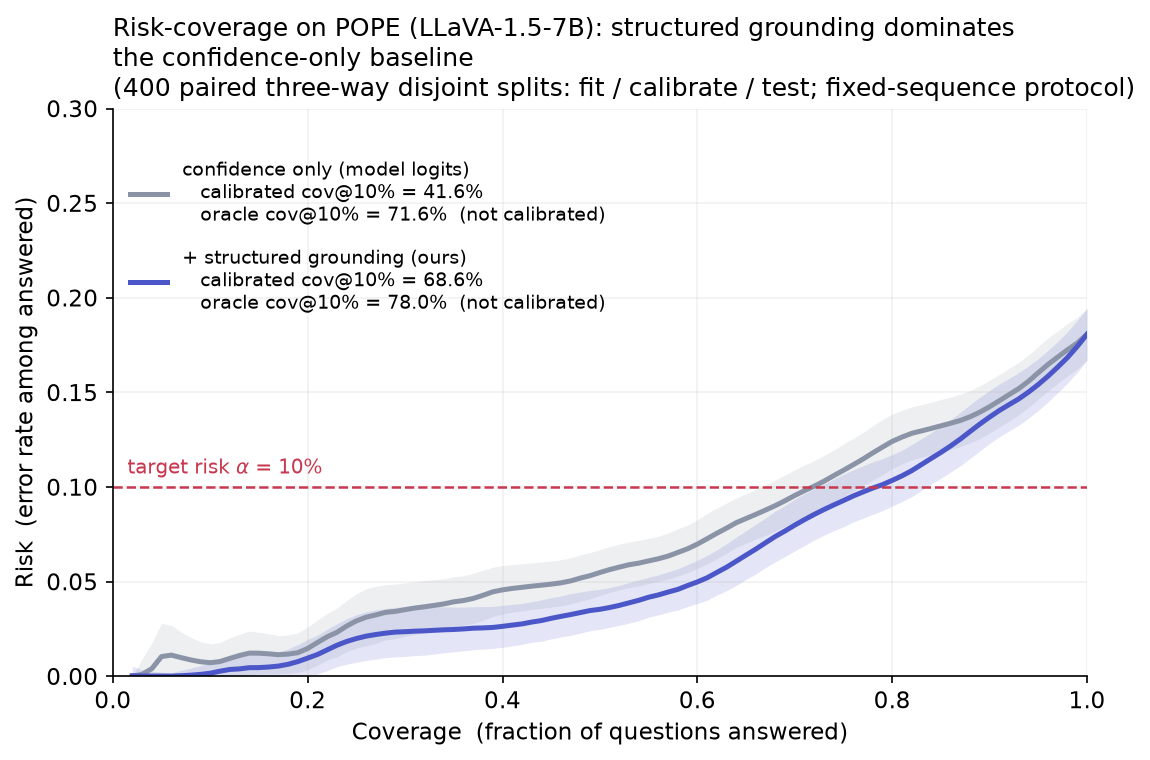
\includegraphics[width=0.72\textwidth]{risk_coverage.png}
\caption{Risk--coverage curves on POPE-1500. The grounded score (blue) lies below the
confidence-only baseline at $99\%$ of coverage levels, meeting it only at full coverage where
both necessarily equal the base risk: lower error for the same coverage, and more coverage for
the same error target. Shaded bands are one standard deviation over $400$ paired three-way
splits; the dashed line marks $\alpha=0.10$. The legend reports two quantities that should not
be confused: \emph{oracle} coverage read off the test-fold curve ($71.6\%\to78.0\%$), and
conformally \emph{calibrated} coverage ($41.6\%\to68.6\%$), the latter being what the tables
report and the gap between them being the price of calibrating rather than knowing. The baseline
is LLaVA's own output logits with no external evidence, which is why it is labelled
``confidence only (model logits)'' rather than ``ConfLVLM-style'':
ConfLVLM's scorer is CLIP image--text similarity, which appears separately as
rung~1 of Table~\ref{tab:attrib} and as the ``$+$ CLIP grounding'' arm of
Figure~\ref{fig:comparison}.}
\label{fig:riskcov}
\end{figure}

\subsection{Composition with the closest concurrent method}
\label{sec:bcea}
Xu et al.~\cite{bcea} rescue borderline claims by acquiring zoomed views and re-scoring the
\emph{original} assertion. Holding the base score fixed and adding one mechanism per arm
(Table~\ref{tab:bcea}), the two mechanisms are complementary: composing them beats every
single-mechanism arm at both risk levels. Re-reading the image and replacing the answer
rescue different claims. We do not claim to beat Xu et al.~\cite{bcea}: our reproduction uses three
coarse crops and under-delivers relative to their published gain at $\alpha=0.10$, so the
defensible conclusion is composition, not superiority.

\begin{table}[t]
\centering
\caption{One common base score, one mechanism added per arm (POPE, LLaVA-1.5, $n=394$
grounded items, $\alpha$ as shown). All arms valid. Composition beats every single mechanism.
This is the one table in the paper at $60$ rather than $\ge400$ paired splits, because the arms
require a re-scoring pass per split; it uses the same fixed-sequence rule as everything else, and
the differences here are large enough that the repetition count is not the binding uncertainty.}
\label{tab:bcea}
\begin{tabular}{lcc}
\toprule
Arm & cov@$0.10$ & cov@$0.15$\\
\midrule
Base filter (confidence only)              & 5.5\%  & 16.5\%\\
\quad + evidence acquisition \citep{bcea}  & 5.5\%  & 24.1\%\\
\quad + detection-grounded score (ours)    & 32.1\% & 63.2\%\\
\quad + certified correction (ours)        & 34.5\% & 71.8\%\\
\textbf{Composed}                          & \textbf{35.8\%} & \textbf{74.2\%}\\
\bottomrule
\end{tabular}
\end{table}

%===============================================================================
\section{A small-calibration failure mode of fixed-sequence testing}
\label{sec:kminfail}

Three results in this paper looked unrelated until we measured the abort rate, and are in fact
one mechanism seen three times. Because it is elementary, checkable in advance, and --- on our
data --- larger than the effect our method is designed to produce, we give it its own section
rather than three scattered paragraphs.

\subsection{The mechanism}

Two facts about the procedure combine badly at small calibration size. The first is
Lemma~\ref{lem:kmin}: with $\alpha=\delta=0.10$ no emitted set smaller than $k_{\min}=22$ items
can be certified at all, and the value is \emph{bound-dependent} --- $22$ for Clopper--Pearson but
$44$, $71$ and $116$ for the betting, empirical-Bernstein and Hoeffding bounds
(Table~\ref{tab:bounds}) --- so a grid start tuned for one bound silently disables another. The
second is that fixed-sequence testing must stop at the \emph{first} non-rejection
(\S\ref{sec:validity}), and the first hypothesis in an ascending sweep is the one with the
smallest emitted set.

Put together: the strictest hypothesis is simultaneously the one with the least statistical power
and the one whose failure costs everything. The arithmetic is stark. Our grid starts at
$\lambda_1=1.5k_{\min}/n_{\mathrm{cal}}$, so the first hypothesis emits $k\approx33$ items, and
Clopper--Pearson at $k=33$ tolerates exactly \textbf{zero} errors:
\begin{align*}
U(0,33;0.10)&=0.0674\le\alpha,\\
U(1,33;0.10)&=0.1128>\alpha,\\
U(2,33;0.10)&=0.1533>\alpha.
\end{align*}
So whenever the top $33$ calibration items by score contain a single error, the whole sequence
returns nothing and the deployed system covers $0\%$. Whether that happens is a property of the
score's extreme upper tail on a $n_{\mathrm{cal}}$-item fold --- not of its average quality, its
AUROC, or the dataset's difficulty.

The condition for this to be fatal rather than merely costly is exactly the one
Remark~\ref{rem:prefix} anticipates: feasibility must be a \emph{prefix} of the grid for
``stop at the first failure'' to lose nothing, and that is risk monotonicity in $\lambda$, which
\S\ref{sec:validity} declines to assume. Where feasibility is not a prefix, the first hypothesis
decides the outcome by itself. On POPE-1500 with raw confidence we can verify this exactly: the
measured first-hypothesis failure rate is $59.2\%$ and the measured abort rate is $59.2\%$ ---
identical, to the split.

The max-over-thresholds rule of \S\ref{sec:exp} hides all of this, because it is free to skip to a
large-$k$ threshold where dozens of errors are tolerable. That is the multiplicity it never pays
for, and the abort column is what appears when the bill is settled.

\subsection{Instance 1: a weak score does not certify a little less, it certifies nothing}

Under a valid fixed sequence, score quality expresses itself almost entirely through the abort
rate rather than through coverage given certification. Raw confidence aborts on $59.2\%$ of
splits and a learned confidence-only score on $32.5\%$, against $0.8\%$ for the same score plus
detection grounding (Table~\ref{tab:score}); the self-consistency baseline of
Table~\ref{tab:selfcons} aborts on $75.2\%$ and self-consistency alone on $100\%$; the
confidence-only arm on VCD-decoded LLaVA aborts on $95.8\%$ (Table~\ref{tab:datasets}); and at
$\alpha=0.05$ even the grounded score aborts on $24.0\%$ (Table~\ref{tab:multialpha}). The claim
this supports is stronger than a coverage claim: the value of an external evidence channel is not
that it buys a few points of coverage but that it makes certification possible at all on between
a third and all of calibration draws.

Two cells in this paper have a $100\%$ abort rate (MME-existence, HallusionBench). Their
certified coverage of $0.0\%$ is the guarantee working exactly as designed --- on HallusionBench
LLaVA is at chance, $\mu\approx0.49$, and Proposition~\ref{prop:floor} forces abstention on at
least $43\%$ of inputs --- but ``$0.0\%$ coverage'' and ``mean coverage $2.6\%$ over splits, of
which $85\%$ are zeros'' are very different statements to a deployer, and only the second is
honest.

\subsection{Instance 2: self-repair is defeated by the prefix, not by the region}

\S\ref{sec:independence} is the same mechanism with a fixed-mass contaminant. The self-repair
block has mass independent of $\lambda$, so at the start of the grid it is the largest fraction
of the emitted set it will ever be, and its $4.9$--$62.4\%$ error rate fails the first hypothesis.
Coverage does not degrade gracefully; it collapses, by $49.3$, $37.3$, $76.9$ and $6.6$ points,
with abort rates of $73.0\%$, $88.8\%$, $98.8\%$ and $25.2\%$ (Table~\ref{tab:selfrepair}). The
budget in \eqref{eq:selfrepair} would in fact be satisfiable at later $\lambda$ on some of these
settings; the test never gets there. Note that the ordering of the four collapse magnitudes is
the ordering of the four abort rates, not the ordering of the four flip-region risks.

\subsection{Instance 3: this, and not headroom, is why CCRC loses on AMBER}

AMBER(d) has $n=228$ items, so a three-way split leaves a $76$-item calibration fold. With
$k_{\min}=22$ the grid starts at $\lambda_1=1.5\times22/76=0.434$ and the first hypothesis again
emits about $33$ items, tolerating zero errors. AMBER's filtering arm clears that bar reliably
because its score is clean at the top: it aborts on $0.00\%$ of splits at both risk levels.
Adding a fixed-mass repair block puts the occasional repair error into that first, smallest,
most fragile hypothesis --- and the fixed sequence must stop there. CCRC aborts on $13.00\%$ and
$12.75\%$ of splits.

Table~\ref{tab:amber} decomposes the reported loss by split class, and the answer is unambiguous.
Conditional on both arms certifying something, CCRC \emph{wins} on AMBER: $+2.17$ points at
$\alpha=0.10$ ($p=6\times10^{-28}$) and $+0.47$ at $\alpha=0.15$ ($p=7\times10^{-30}$). The
splits on which CCRC aborts and filtering does not --- $52$ of $400$ --- contribute $-12.09$
points, which is $119\%$ of the entire reported loss at $\alpha=0.10$ and $103\%$ at
$\alpha=0.15$. Every other split class contributes positively. And the dilution direction is
favourable throughout: $r_r=3.60\%<r_a=4.53\%$ at $\alpha=0.10$ and $0.00\%<7.45\%$ at
$\alpha=0.15$, so the ``repairs consume slack'' branch of Proposition~\ref{prop:dilution} ---
the branch a headroom explanation requires --- is not the branch AMBER is in.

\begin{table}[t]
\centering
\caption{The AMBER(d) loss, decomposed ($400$ paired splits, $q=0.10$). The unconditional gain
is what Table~\ref{tab:ccrc} reports and what a deployer experiences. The conditional gain is
what CCRC does when it certifies at all. The gap is entirely one split class. POPE-1500 is shown
for contrast: there, CCRC never aborts and filtering occasionally does --- the mirror image.}
\label{tab:amber}
\small
\resizebox{\textwidth}{!}{%
\begin{tabular}{lcccc}
\toprule
& \multicolumn{2}{c}{AMBER(d), $n=228$} & \multicolumn{2}{c}{POPE-1500, $n=1500$}\\
\cmidrule(lr){2-3}\cmidrule(lr){4-5}
& $\alpha=0.10$ & $\alpha=0.15$ & $\alpha=0.10$ & $\alpha=0.15$\\
\midrule
unconditional gain (Table~\ref{tab:ccrc}) & $-10.20$ & $-11.90$ & $+3.18$ & $+1.95$\\
gain $\mid$ neither arm aborts & $\mathbf{+2.17}$ & $\mathbf{+0.47}$ & $+2.68$ & $+1.95$\\
\quad ($95\%$ CI) & $[+1.8,+2.5]$ & $[+0.4,+0.5]$ & --- & ---\\
abort rate, filtering & 0.00\% & 0.00\% & 0.75\% & 0.00\%\\
abort rate, CCRC & \textbf{13.00\%} & \textbf{12.75\%} & \textbf{0.00\%} & \textbf{0.00\%}\\
$\hat\lambda$ moves & 15.2\% & 1.7\% & 28.0\% & 23.5\%\\
$r_a$ / $r_r$ & 4.53 / \textbf{3.60}\% & 7.45 / \textbf{0.00}\% & 7.96 / 0.24\% & 12.65 / 0.32\%\\
dilution direction & favourable & favourable & favourable & favourable\\
\midrule
\multicolumn{5}{l}{\emph{contribution to the $-10.20$ at $\alpha=0.10$, by split class:}}\\
\quad both certify ($348$ splits) & $+1.89$ & & &\\
\quad \textbf{CCRC aborts, filter does not ($52$)} & $\mathbf{-12.09}$ & & &\\
\quad filter aborts, CCRC does not ($0$) & $+0.00$ & & &\\
\bottomrule
\end{tabular}
}
\end{table}

The effect does not vanish over AMBER's available range of $n$. In a separate subsampling sweep
at lower repetition count --- which is why its full-size level differs slightly from
Table~\ref{tab:amber}'s --- the CCRC abort rate is $11.0\%$ at $n=228$, $10.2\%$ at $190$,
$9.2\%$ at $152$ and $61.9\%$ at $114$: what binds is the interaction of fold size with the grid
start rather than $n$ alone. And the same probe run on
POPE confirms that AMBER is not special: subsampled to $n=228$, CCRC loses $3.65$ points on POPE
too, with abort rates of $43.5\%$ (filtering) and $53.8\%$ (CCRC). The setting that loses is the
setting with the smallest calibration fold, on either dataset.

\paragraph{What this changes, and what it costs us.}
It costs us our only claimed instance of Conjecture~\ref{conj:headroom}, which is why that
statement is now labelled a conjecture with no confirming evidence. It also costs us the clean
story in which a checkable precondition screens deployments in advance. What replaces it is a
different check, also computable before calibration and considerably better supported: given
$n_{\mathrm{cal}}$, $\alpha$ and $\delta$, compute $k_{\min}$ and the emitted count at the grid
start, ask how many errors the bound tolerates there, and ask whether the score's upper tail is
clean enough to supply that. If the answer is ``zero errors tolerated'' --- which it is for any
$n_{\mathrm{cal}}\lesssim500$ at $\alpha=\delta=0.10$ --- then \emph{any} perturbation of the
strictest hypothesis, including a beneficial one, is a coin flip on the whole deployment. The
practical remedies are equally elementary: a larger calibration fold, a looser $\alpha$, or a
grid start chosen so the first hypothesis tolerates at least one error. We flag rather than
implement the last, because choosing it from data would need its own share of $\delta$.

%===============================================================================
\section{A sequential failure mode}
\label{sec:sequential}

Correction is more attractive in free-form generation than in yes/no answering: replacing a
hallucinated word preserves a caption that deletion would mutilate. The extension looks
mechanical --- decompose the caption into claims, repair the unsupported ones, continue
decoding --- and two obstacles are already known. Editing a prefix makes later tokens
off-policy, which is feedback covariate shift rather than exogenous shift
\citep{fannjiang2022fcs}, so weighted conformal methods \citep{tibshirani2019} do not apply.
And per-claim guarantees say nothing about a whole sequence, whose length is itself
data-dependent.

Both could in principle be handled. Prefix-conditional (Mondrian) $p$-values make each
decision valid given the realised prefix, so how we arrived there --- including by our own
edits --- is absorbed into the conditioning; e-processes with Ville's inequality give
sequence-level anytime validity, and are robust to adaptive intervention because our
corrections are predictable with respect to the decoding filtration
\citep{waudbysmith2024,ramdas2023}. The residual difficulty is that the calibration pool
drifts, since the deployed policy writes different text. The natural fix is on-policy
calibration by iteration to a fixed point, and its convergence argument requires the
correction map to be monotone. We measured whether it is, before attempting a proof.

\paragraph{Design.}
For each image we generate a caption greedily, locate the first hallucinated object mention
at position $t$ using AMBER's per-image present/absent object lists, and construct two
prefixes \emph{identical up to $t$}: one retaining the hallucinated word, one substituting
the best-detected object the image genuinely contains. We then continue decoding the same
number of tokens from each prefix and count hallucinated mentions in the continuations
only. Matched prefixes make the contrast causal: the only difference between the two
continuations is the intervention.

\paragraph{Result.}
Repair makes the continuation worse (Table~\ref{tab:monotone},
Figure~\ref{fig:monotonicity}). Downstream hallucinated mentions rise from $1.207$ to
$1.413$, a paired difference of $+0.2066\pm0.0908$ ($n=121$, $t(120)=2.27$, two-sided
$p=0.025$), with $45$ cases worsening against $25$ improving and $51$ tied. The sign is
supported by three tests that make different assumptions --- paired $t$ $p=0.025$, Wilcoxon
signed-rank $p=0.035$, exact sign test $p=0.023$, all two-sided --- which is the robustness
evidence that matters given that $42\%$ of pairs are tied. (Because of those ties the
rank-based Hodges--Lehmann location estimate is exactly $0.000$ even though the mean and every
test statistic are positive; we state that rather than let a reader discover it.)

\begin{table}[t]
\centering
\caption{Paired matched-prefix test of monotonicity ($n=121$ cases). Repair increases
hallucination in the continuation. All $p$-values two-sided.}
\label{tab:monotone}
\resizebox{\textwidth}{!}{%
\begin{tabular}{lccc}
\toprule
Downstream measure (continuation only) & Original & Repaired & paired diff.\ ($p$)\\
\midrule
Hallucinated mentions (mean)      & 1.207 & \textbf{1.413} & $+0.207$ ($0.025$)\\
Hallucinations per $100$ words    & 3.61  & 4.30  & $+0.75$ ($0.011$)\\
Faithful mentions (mean)          & 1.579 & 1.752 & $+0.174$ ($0.077$)\\
Continuation length (words)       & 33.4  & 32.9  & $-0.55$ ($0.092$)\\
Hallucinated share of mentions    & 0.433 & 0.447 & $-0.004$ ($0.884$)\\
\midrule
\multicolumn{4}{l}{Primary endpoint: $+0.2066\pm0.0908$; $t(120)=2.27$, $p=0.025$; Wilcoxon
$p=0.035$; sign test $p=0.023$}\\
\multicolumn{4}{l}{$95\%$ CI $[+0.027,+0.386]$; Cohen's $d_z=0.207$; Hodges--Lehmann $+0.000$}\\
\multicolumn{4}{l}{Cases better / worse / tie: $25$ / $45$ / $51$}\\
\bottomrule
\end{tabular}
}
\end{table}

\begin{figure}[t]
\centering

\includegraphics[width=\textwidth]{fig_monotonicity.png}
\caption{(A) Mean hallucinated mentions in the continuation after keeping versus repairing
the flagged claim; error bars are standard errors. (B) Distribution of the paired
difference; mass to the right of zero indicates repair worsening the continuation. The
effect is modest in size and its sign is what matters for the theory; \S\ref{sec:power} bounds
how little the experiment says about its magnitude.}
\label{fig:monotonicity}
\end{figure}

\subsection{How much this experiment can support}
\label{sec:power}

The primary result is significant at conventional levels under three tests, and it is also
under-powered. Both are true, and the second decides what may be concluded: the fixed-point route
is not \emph{closed} by this evidence, it is \emph{unsupported} by it. The numbers, at the
observed paired standard deviation of $0.9993$ with $n=121$:

\begin{itemize}
\item The two-sided minimum detectable effect at $80\%$ power is $+0.2566$, which is
\emph{larger} than the observed $+0.2066$. The study was designed to detect effects of at least
about a quarter of a hallucinated mention and detected a smaller one, which is a
marginally-powered positive rather than a well-powered one.
\item Achieved power at the observed effect is $61.6\%$; $186$ pairs ($65$ more) would be needed
for $80\%$ power at this effect size, and $248$ for $90\%$. (Post-hoc achieved power is a
monotone restatement of the $p$-value and is not evidence about the true effect; we report it
because it is the number most readers will want and the MDE is the one that carries information.)
\item Equivalence testing bounds the effect from the other side. Against a pre-specified margin
of $\pm0.25$ --- a quarter of a hallucinated object per repair, roughly $20\%$ of the baseline ---
TOST does \emph{not} establish equivalence ($p=0.317$). The smallest margin we can establish at
the $5\%$ level is $\Delta=0.357$, i.e.\ $29.6\%$ of baseline.
\item So the experiment simultaneously rules out an exact null, rules out true effects larger in
magnitude than $0.357$, and cannot distinguish $+0.207$ from anything in $[+0.027,+0.386]$ --- a
fourteen-fold range. \textbf{The increase is established as a sign, not as a magnitude.}
\end{itemize}

What survives is exactly what the theory needs and no more. A monotone fixed-point argument
requires the correction map to be non-increasing in downstream risk; a sign is enough to withdraw
support from that, and a magnitude would be required only to price the cost, which we therefore do
not attempt to price. The right statement is: \emph{our data does not support the monotonicity
property a fixed-point calibration argument would rest on, and settling the question would take
$n\ge186$ matched pairs.} We do not claim the route is closed, and any downstream use of the
number $0.207$ as a quantity rather than as a direction is unsupported by this experiment.

We also pin down the per-word figure quoted in Table~\ref{tab:monotone}, since three defensible
variants of it exist. The paired per-item rate difference over the $119$ pairs with non-empty original
continuations is $+0.0075$ per word ($95\%$ CI $[+0.0017,+0.0132]$, two-sided paired $p=0.011$);
the pooled ratio-of-totals is $+0.0069$ (paired-cluster bootstrap $p=0.0086$). Including the two
degenerate pairs whose original continuation is empty raises the estimate to $+0.0115$ and the
$p$-value to $0.023$, because one of them contributes $+0.5$ on a two-word continuation and
supplies a third of the numerator. We report the $119$-pair version, state the exclusion rule, and
note that the result is not robust to those two pairs.

\paragraph{What this rules out, and what it does not.}
Because the correction map is not non-increasing on this evidence, monotone convergence arguments
of Knaster--Tarski type have no basis here and we do not claim a sequential guarantee of that
form. What survives is a coupling bound, which is weaker but assumption-light.

For a sequence of claims $O=(o_1,\dots,o_T)$ let $\Risk(O)=\E[\,\#\{t:o_t\text{ false}\}\,]$
be the expected count of false claims, the quantity a CHAIR-style loss charges for. Two
regimes must be separated, and the distinction is exactly what \S\ref{sec:sequential}
measures.

\begin{theorem}[Coupling bound for corrected outputs]
\label{thm:coupling}
Let $O$ denote the original output and $O'$ the output after a repair rule is applied to a
region $R$, and suppose the repair is \emph{non-interfering}: conditional on not being
repaired, every claim's truth value is unchanged by repairs elsewhere. Then
\[
\Risk(O')\ \le\ \Risk(O)\;+\;\Pr[X\in R]\cdot\Pr[\text{repair wrong}\mid X\in R].
\]
Without non-interference the bound acquires a third term,
\begin{equation}
\label{eq:interference}
\Risk(O')\ \le\ \Risk(O)\;+\;\Pr[X\in R]\cdot\Pr[\text{repair wrong}\mid X\in R]\;+\;\Iota,
\end{equation}
\begin{equation*}
\Iota \;:=\; \E\big[\Delta_{R^c}\big],
\end{equation*}
where $\Delta_{R^c}$ is the change in the number of false claims outside $R$ induced by
repairing inside it.
\end{theorem}

\begin{proof}
Decompose by whether a claim is repaired. Under non-interference the claims in $R^c$ retain
their truth values, contributing at most $\Risk(O)$; on $R$ the emitted claim is wrong only
if the repair is wrong, contributing at most
$\Pr[X\in R]\Pr[\text{repair wrong}\mid X\in R]$. Summing gives the first bound. In general
the $R^c$ contribution is $\Risk(O)+\E[\Delta_{R^c}]$ by definition of $\Delta_{R^c}$, which
gives \eqref{eq:interference}.
\end{proof}

\begin{remark}[The interference term is not negligible here]
\label{rem:interference}
Non-interference is the assumption \S\ref{sec:sequential} falsifies: we measure
$\widehat{\Iota}=+0.207\pm0.091$ additional false claims per repair ($n=121$, $p=0.025$), so
for a single repair the interference term is roughly the same size as the direct repair-error
term and cannot be dropped. Any procedure certifying corrected sequences must estimate
$\Iota$ rather than assume it away, and $\Iota$ depends on the repair rule --- which is why
a context-aware rule is the natural next step rather than a tighter bound.
\end{remark}

\begin{remark}[What the corollary does and does not give]
\label{rem:corollary}
Controlling $\Risk(O)\le\alpha_1$ and the repair term by $\alpha_2$ at confidence
$1-\delta/2$ each yields $\Risk(O')\le\alpha_1+\alpha_2+\Iota$ at confidence $1-\delta$. We
flag a limitation of this composition rather than hiding it: certifying $\Risk(O)$ for the
\emph{uncorrected} generation is precisely the object the abstention floor makes expensive,
so the corollary is useful only relative to an already-selective base policy (for which
$\Risk$ is conditioned on emission), not to raw generation. Making the sequential guarantee
self-contained --- certifying the corrected sequence without first certifying the
uncorrected one --- remains open.
\end{remark}

\paragraph{What this implies for algorithm design.}
The measurement identifies a cost that a myopic procedure does not charge for. Greedy per-claim
repair optimises the risk of the claim in front of it while imposing an additional hallucinated
claim on the continuation with probability we can sign but not size. A correct sequential
procedure must therefore price the \emph{continuation}, not the claim --- for instance by
searching over rewrite trajectories under an accumulated risk ledger rather than deciding each
claim independently. \S\ref{sec:discussion} states why that is a genuinely different statistical
object and why we regard it as the main open problem this paper leaves.

\paragraph{A competing explanation, and what survives it.}
Table~\ref{tab:monotone} contains rows that complicate the headline. Repair raises
faithful mentions by $+0.174$ ($p=0.077$) at the same time as it raises hallucinated mentions by
$+0.207$, in continuations that are slightly \emph{shorter} ($33.4\to32.9$ words, $p=0.092$).
Repaired prefixes therefore produce denser object talk --- mention density rises about $15\%$ in
relative terms --- and the obvious alternative reading is that correction makes the continuation
more descriptive rather than less faithful. Two normalisations settle it. Per word, hallucination
rises significantly ($+0.0075$ per word, two-sided $p=0.011$). Per \emph{mention}, it does not
move at all: the hallucinated share of mentions goes $0.433\to0.447$ pooled, and the paired
difference is $-0.0039$ ($p=0.884$, $n=111$ pairs with mentions in both arms). The competing
explanation is therefore substantially correct as a description of \emph{why} the count rises.

It does not, however, rescue the monotonicity argument, and the reason is that the quantity
being certified is a count and not a ratio. A CHAIR-style risk charges for each hallucinated
mention emitted; a procedure that repairs one claim and emits two additional false ones has
increased the risk of its own output regardless of how many true claims came with them. What
the normalised results do establish is the mechanism --- repair perturbs the generation
towards denser description, and hallucination scales with density --- and that a
density-controlled repair rule might avoid the cost. We report the share result because a
reader is entitled to it, and because it makes the negative result narrower than the raw
count suggests.

\paragraph{Scope of the negative result.}
Our repair substitutes the globally best-detected object, which can be contextually
inappropriate mid-sentence and may push the prefix off-policy for reasons unrelated to
faithfulness. The supported claim is that \emph{context-blind} substitution carries a
downstream cost in absolute and per-word terms, not that all correction must, and not that
it degrades the faithful/hallucinated \emph{balance}. Constraining repairs to the model's
own top-$k$ continuations --- which the one-shot procedure of \S\ref{sec:method} already
implies --- is the natural remedy and remains to be tested.

%===============================================================================
\section{Ablations}
\label{sec:ablations}

\subsection{The score combiner, and a validity trap}

Channel 1 is a learned function of a handful of scalars. It is natural to ask whether a
more expressive combiner helps. It does not, and it can silently invalidate the guarantee.

Table~\ref{tab:combiner} reports two protocols, and the audit statistic is the exceedance
fraction rather than mean risk. Under the naive protocol, where the combiner is fitted on the
same fold used to calibrate the threshold, gradient boosting and random forests appear to
certify far more coverage --- $89.2\%$ and $86.1\%$ --- but $93.5\%$ and $72.5\%$ of their splits
\emph{exceed} the risk target on held-out data. Their mean realised risks, $13.3\%$ and $12.1\%$,
badly understate that: the exceedance fraction is the guarantee actually being
broken. The mechanism is straightforward: a high-capacity model overfits
the calibration scores, so empirical error on the calibration fold understates true error and the
threshold is set too permissively. (Note that under this protocol the full-item-set exceedance is
\emph{not} a valid proxy --- two thirds of those items were used to fit the score, so random
forest looks fine at $6.8\%$ there while failing at $72.5\%$ on held-out data. Where fit and
calibration overlap, only the held-out column may be read.)

Under a three-way split all combiners are valid --- but they are \emph{not} tied. Logistic
regression beats gradient boosting by $11.90$
points ($p=8\times10^{-18}$) and random forest by $15.41$ points ($p=2\times10^{-20}$), and the
reason is again the abort rate: $14.5\%$ and $24.8\%$ of splits against logistic regression's
$0.0\%$. A high-capacity score here is not merely no better; it fails the first hypothesis of the
fixed sequence on up to a quarter of splits. The MLP is worse still, $14.2\%$ mean coverage with
a $60.8\%$ abort rate, from overfitting six features.

\begin{table}[t]
\centering
\caption{Combiner ablation on POPE-1500 ($\alpha=\delta=0.10$, $400$ paired repetitions, six
features). The audit column is $\Pr[\text{realised risk}>\alpha]$, not mean risk. Under data
reuse, high-capacity combiners \emph{break} the guarantee on the majority of splits; under a
three-way split they are valid but abort. Logistic regression is chosen deliberately, and the
abort column is the reason.}
\label{tab:combiner}
\footnotesize
\resizebox{\textwidth}{!}{%
\begin{tabular}{lcccccc}
\toprule
& \multicolumn{2}{c}{Naive: fit $=$ calibrate} & \multicolumn{4}{c}{Three-way split}\\
\cmidrule(lr){2-3}\cmidrule(lr){4-7}
Combiner & cov@$10\%$ & $\widehat{\Pr}[\Risk>\alpha]$ (test fold) & cov@$10\%$ & abort
& $\widehat{\Pr}[\Risk>\alpha]$ (all items) & vs.\ logistic\\
\midrule
Logistic regression & 74.3\% & 18.5\% & \textbf{70.7\%} & \textbf{0.0\%} & 3.2\% & ---\\
Gradient boosting   & 89.2\% & \textbf{93.5\%} (violated) & 58.8\% & 14.5\% & 0.0\% & $-11.90$\\
Random forest       & 86.1\% & \textbf{72.5\%} (violated) & 55.3\% & 24.8\% & 0.3\% & $-15.41$\\
MLP $(64,32)$       & 25.6\% & 14.9\% & 14.2\% & 60.8\% & 1.3\% & $-56.49$\\
\bottomrule
\end{tabular}
}
\end{table}

We draw two conclusions. Practically, the score must be fitted on a fold disjoint from
calibration --- a discipline that costs $3.6$ points of coverage for logistic regression and
$30$ points for the tree ensembles, and is necessary for any scorer whose capacity is not
negligible. Conceptually, capacity is not the bottleneck: the features are already informative
scalars, and what limits efficiency is the quality of the grounding signal, not the flexibility
of the combiner --- with the addendum that excess capacity is not free but actively harmful under
a valid sequential test.

\subsection{The risk bound}

The emitted-set error is a binomial proportion, so an exact interval should dominate
general-purpose concentration inequalities, and it does: at $\alpha=0.10$ Clopper--Pearson
certifies $70.7\%$ coverage, the betting bound $62.5\%$, empirical Bernstein $23.2\%$ and
Hoeffding $18.8\%$ (Table~\ref{tab:bounds}). All four are valid; the loose two are simply
conservative, realising $3.2\%$ and $4.2\%$ risk against a $10\%$ budget. This is consistent with
the hierarchy established by Kotte~\cite{crcimposs} and indicates that for binary losses the choice of
bound is worth more than fifty points of coverage. The $k_{\min}$ column is the same story from
the other end and is the one to check before choosing: at $\alpha=\delta=0.10$ Hoeffding cannot
certify an emitted set smaller than $116$ items, so on a $76$-item calibration fold it cannot
certify anything at all whatever the score does. Variance-adaptive or betting-style bounds
\citep{waudbysmith2024} become preferable for graded losses, which is the natural setting for
claim-level factuality scores.

\begin{table}[t]
\centering
\caption{Risk-bound ablation (POPE-1500, three-way split, $400$ repetitions). Exact binomial
dominates for a binary loss; the others are valid but conservative. $k_{\min}$ is the smallest
emitted set the bound can certify with zero observed errors (Lemma~\ref{lem:kmin}), which is a
pre-calibration screening quantity: a bound whose $k_{\min}$ exceeds what the grid start can emit
certifies nothing. The audit column is the fraction of splits whose risk on all items exceeds
$\alpha$, against $\delta=0.10$.}
\label{tab:bounds}
\resizebox{\textwidth}{!}{%
\begin{tabular}{lccccccc}
\toprule
& & \multicolumn{3}{c}{$\alpha=0.10$} & \multicolumn{3}{c}{$\alpha=0.15$}\\
\cmidrule(lr){3-5}\cmidrule(lr){6-8}
Upper confidence bound & $k_{\min}$ & cov & risk & $\widehat{\Pr}[\Risk>\alpha]$
                                    & cov & risk & $\widehat{\Pr}[\Risk>\alpha]$\\
\midrule
Hoeffding                & 116 & 18.8\% & 4.2\% & $0\%$ & 75.8\% & 9.4\%  & $0\%$\\
Empirical Bernstein      &  71 & 23.2\% & 3.2\% & $0\%$ & 70.3\% & 8.8\%  & $0\%$\\
Betting (e-CRC)          &  44 & 62.5\% & 5.9\% & $0\%$ & 78.1\% & 9.9\% & $0\%$\\
Clopper--Pearson (exact) &  22 & \textbf{70.7\%} & 7.8\% & $3\%$ & \textbf{86.1\%} & 12.5\% & $2\%$\\
\bottomrule
\end{tabular}
}
\end{table}

\subsection{Positioning summary}

Figure~\ref{fig:comparison} summarises where CCRC sits. Panel A gives risk--coverage curves;
panel B contrasts capabilities across recent methods. Mitigation methods
\citep{opera,attnlens,reverse} operate only at full coverage and offer no guarantee;
conformal methods \citep{conflvlm,onlineabstention} guarantee but only delete or abstain;
Xu et al.~\cite{bcea} re-scores without changing the answer. CCRC is, to our knowledge, the first to
certify an output that differs from the model's --- while requiring, as
\S\ref{sec:independence} shows, an independent channel to do so in practice.

\begin{figure}[t]
\centering

\includegraphics[width=\textwidth]{comparison_figure.png}
\caption{(A) Risk--coverage on POPE-1500 for the three score variants, $400$ paired three-way
splits, with oracle and conformally calibrated coverage at $\alpha=0.10$ labelled separately in
the legend. (B) Capability comparison with recent methods. Mitigation approaches change the base
model but provide no guarantee; existing conformal approaches guarantee but only remove or
abstain; Xu et al.~\cite{bcea} guarantees and acquires evidence but does not change the emitted answer.
Our layer composes on top of mitigation decoders (\S\ref{sec:vcd}).}
\label{fig:comparison}
\end{figure}

%===============================================================================
\section{Discussion}
\label{sec:discussion}

\paragraph{What the results support.}
Permitting a selective predictor to emit a substituted answer is a real degree of freedom: it
evades the premise of Proposition~\ref{prop:floor}, the guarantee survives the substitution
(Theorem~\ref{thm:validity}) because risk control cares about error indicators rather than about
provenance, and in eight of ten cells it converts a repaired mass of $1$--$2\%$ into $+0.4$ to
$+7.6$ points of certified coverage with intervals excluding zero. The mechanism is understood
well enough to be decomposed: most of that is the repaired items being emitted at almost no risk
cost, and $+0.2$ to $+1.8$ points is genuine dilution.

\paragraph{What they do not.}
The gains are modest and conditional. The mechanism requires a strict gate
(Table~\ref{tab:qsens}), an independent channel (\S\ref{sec:independence}), and a calibration
fold large enough that the first hypothesis of the fixed sequence can pass
(\S\ref{sec:kminfail}) --- and the last of these costs us more on the setting where it binds than
the mechanism gains anywhere. What we do \emph{not} have is a clean headroom precondition:
Conjecture~\ref{conj:headroom} has no confirming instance
in our data. Most of our margin over a published baseline is the correctness score rather than
the algorithm --- $64.5$ points against $2.3$ (Table~\ref{tab:attrib}) --- and the closest
concurrent method is complementary rather than dominated (Table~\ref{tab:bcea}). The one-shot
theory is a correct but standard application of fixed-sequence testing with exact bounds, and it
is stated for a value-indexed family while our measurements come from the rank-indexed variant
(Remark~\ref{rem:rankvsvalue}). The interesting theory is sequential, and
\S\ref{sec:sequential} shows that we cannot currently support the most natural route to it.

\paragraph{Limitations.}
Channel 2 is an object detector, so the evaluated method addresses existence hallucination ---
and, within that, only \emph{missed} objects: \S\ref{sec:symgate} shows that even a
polarity-symmetric gate corrects no false-positive existence hallucination in any setting,
because on the negative side the reachable items are the ones the model already gets right. On
attribute-, counting- and reasoning-heavy benchmarks the method degenerates to filtering, which
remains valid but gains nothing. The independence of channel 2 is an assumption, and our own
instantiation violates it (channel 1's features include the detector score); a detector sharing
the VLM's blind spots would weaken certification without invalidating it. The repair gate $q$ is
fixed a priori rather than learned; \S\ref{sec:qsel} prices what that choice is worth and
Appendix~\ref{app:qdelta} gives a fully valid alternative. Exchangeability is assumed throughout;
under deployment shift the stated level need not hold, and adaptive conformal methods
\citep{gibbs2021} would be required. Our sequential experiment uses one backbone, a context-blind
repair rule, and $n=121$ pairs, which is under-powered as a magnitude claim
(\S\ref{sec:power}). And every interval in this paper is over splits of a fixed dataset, so none
of them speaks to replication on new items.

\paragraph{Outlook.}
The open problem we consider most interesting is the one the sequential negative result exposes.
Because repairing a claim changes which subsequent claims exist, a sequential procedure faces an
endogenous item set and must select among rewrite trajectories rather than filter a fixed list.
Selecting the best trajectory and then reporting its certificate is a selective-inference error,
so a correct procedure needs a certificate simultaneous over the search tree. Settling whether
repair degrades continuations at all would take $n\ge186$ matched pairs; building the
simultaneous certificate is the larger task. A second, cheaper item: the failure mode of
\S\ref{sec:kminfail} suggests that fixed-sequence testing is the wrong search strategy at small
calibration size, and that a method spending a little $\delta$ to avoid staking everything on the
strictest hypothesis would dominate it exactly where our method currently loses.

\section{Conclusion}

Selective prediction for vision--language models is expensive because of a bound whose
premise --- that the emitted answer is the model's own --- is an assumption about the action
space rather than about the data. Relaxing it works, but not freely and not by much: certified
correction requires an independent evidence channel, a strict repair gate, and a calibration fold
large enough for the sequential test to get started, and what it delivers is a couple of points
of certified coverage against the sixty-odd that the correctness score delivers. Applied
myopically in generation, the same idea makes things measurably worse. We have tried to report the
conditions and the failures as carefully as the improvements --- including the ones that cost us a
proposition, a multiplier and a diagnosis --- in the belief that for methods whose selling point
is a guarantee, the boundaries of that guarantee are the substance of the contribution.

\subsubsection*{Broader Impact Statement}
Attaching guarantees to model outputs can improve safety, but a guarantee is only as
meaningful as its assumptions. Our procedure controls the error rate among emitted answers
under exchangeability and requires a genuinely independent evidence channel; if either
fails --- under deployment shift, or with a detector sharing the model's blind spots --- the
stated level may not hold. Emitting a \emph{corrected} answer also changes the failure mode
presented to a user, replacing an abstention that invites scrutiny with a confident
substitution that may not. For this reason we regard the checkable precondition and the
sequential negative result as safety-relevant components of the contribution rather than
limitations to be minimised, and we recommend that any deployment verify the precondition
and monitor channel independence rather than treating the nominal $\alpha$ as a guarantee
that transfers unconditionally.
\appendix
\section{Additional results}

\subsection{Synthetic validation of the three pillars}
\label{app:synth}
Before any real-data experiment we validated the procedure on synthetic data where ground
truth is controllable, confirming (i) that the certified risk is respected, (ii) that a
better-separated score buys coverage at fixed risk, and (iii) that a single global
threshold can satisfy a marginal guarantee while violating it on a minority subgroup
($25.3\%$ realised risk against a $10\%$ target), which group-conditional (Mondrian)
calibration repairs ($9.8\%$ and $9.7\%$ on the two groups). The last point motivates
treating conditional coverage as a separate requirement from marginal coverage; we report it
on synthetic data only, as our real-data samples are not category-balanced.

A second synthetic study is the one Remark~\ref{rem:rankvsvalue} relies
on: it fixes a known $\Pr[Y=1\mid s]$ so that the population risk of any selected threshold can
be computed by quadrature rather than estimated, and measures the exceedance of the
\emph{rank}-indexed fixed sequence --- the variant we implement, and the one the theorem does not
cover --- over four score shapes $\times$ four calibration sizes at $4000$ replications per cell.
Unconditional exceedance is $0.0$--$5.9\%$ against $\delta=0.10$ in all sixteen cells. The
simulation also reproduces \S\ref{sec:kminfail} from first principles: abort rates run from $1\%$
to $100\%$ across the grid and are governed by how fast $\Pr[Y=1\mid s]$ rises in the extreme
upper tail, not by the score's average separability.

\subsection{Multi-$\alpha$ table}
Table~\ref{tab:multialpha} gives certified coverage at four risk levels, the numerical
version of Figure~\ref{fig:covalpha}. The abort block is the part worth reading: at
$\alpha=0.05$, $k_{\min}=45$ and two thirds of splits certify nothing on the confidence-only
score.

\begin{table}[h]
\centering
\caption{Certified coverage and abort rate at four risk targets (POPE-1500, LLaVA-1.5, $400$
paired splits). $k_{\min}$ is $45$, $22$, $15$, $11$ at the four targets. Gains over
confidence-only are paired; all exclude zero except CLIP at $\alpha=0.20$ ($-0.06$, $p=0.27$),
which is why ``the grounded score dominates at every level'' is stated in
\S\ref{sec:score} for detection grounding only.}
\label{tab:multialpha}
\begin{tabular}{lcccc}
\toprule
Score & $\alpha=0.05$ & $0.10$ & $0.15$ & $0.20$\\
\midrule
\multicolumn{5}{l}{\emph{certified coverage}}\\
Confidence only         & \phantom{0}9.0\% & 41.6\% & 81.4\% & 97.3\%\\
$+$ CLIP grounding      & 13.9\% & 63.4\% & 82.5\% & 97.2\%\\
$+$ detection grounding & \textbf{27.3\%} & \textbf{68.6\%} & \textbf{86.4\%} & \textbf{97.7\%}\\
\midrule
\multicolumn{5}{l}{\emph{abort rate}}\\
Confidence only         & 65.8\% & 32.5\% & 0.0\% & 0.0\%\\
$+$ CLIP grounding      & 49.8\% & \phantom{0}0.5\% & 0.0\% & 0.0\%\\
$+$ detection grounding & \textbf{24.0\%} & \phantom{0}\textbf{0.8\%} & 0.0\% & 0.0\%\\
\midrule
\multicolumn{5}{l}{\emph{paired gain of detection grounding over confidence only}}\\
& $+18.29$ & $+27.01$ & $+5.03$ & $+0.48$\\
\bottomrule
\end{tabular}
\end{table}

\subsection{Validity audit, all cells}
\label{app:audit}
Table~\ref{tab:audit} is the audit referred to throughout: the fraction of splits whose realised
risk exceeds $\alpha$, against $\delta=0.10$, for every setting $\times$ risk level $\times$ arm.
The column that decides the question is \texttt{exc(all)}, the selected policy re-scored on all
$n$ items, which is a low-noise proxy for its population risk; \texttt{exc(te)} is the same
statistic on the $n/3$ held-out fold and is inflated by binomial noise at that size. Aborted
splits emit nothing and are excluded from the denominators.

\begin{table}[h]
\centering
\caption{Validity audit over all $40$ cells ($400$ paired splits each). Every cell satisfies
$\texttt{exc(all)}\le\delta=0.10$. Ranges: \texttt{exc(all)} $0.0$--$5.1\%$, \texttt{exc(te)}
$3.1$--$22.3\%$.}
\label{tab:audit}
\small
\resizebox{\textwidth}{!}{%
\begin{tabular}{lcccccccc}
\toprule
& & \multicolumn{2}{c}{filtering} & \multicolumn{2}{c}{$q=0.10$}
& \multicolumn{2}{c}{$q=0.25$} & $q=0.50$\\
\cmidrule(lr){3-4}\cmidrule(lr){5-6}\cmidrule(lr){7-8}\cmidrule(lr){9-9}
Setting & $\alpha$ & te & all & te & all & te & all & te / all\\
\midrule
POPE-1500 LLaVA    & 0.10 & 14.9 & 3.5 & 14.5 & 3.5 & 15.2 & 3.1 & 15.5 / 2.8\\
POPE-1500 LLaVA    & 0.15 & 15.5 & 3.2 & 14.2 & 2.0 & 15.5 & 2.8 & 15.2 / 2.8\\
POPE-adv LLaVA     & 0.10 & 10.8 & 2.5 & 10.6 & 3.3 & 15.3 & 4.0 & 16.6 / 3.7\\
POPE-adv LLaVA     & 0.15 & 14.1 & 0.8 & 12.6 & 1.5 & 12.5 & 1.3 & 12.9 / 1.5\\
POPE-adv Qwen2-VL  & 0.10 & 16.0 & 1.8 & 15.4 & 1.8 & 17.0 & 3.0 & 17.6 / 3.6\\
POPE-adv Qwen2-VL  & 0.15 & 10.5 & 0.0 & \phantom{0}9.8 & 0.0 & \phantom{0}9.9 & 0.0 & \phantom{0}9.8 / 0.0\\
POPE-adv LLaVA+VCD & 0.10 & 13.0 & 1.9 & 12.2 & 2.3 & 16.3 & 3.1 & \textbf{22.3} / \textbf{5.1}\\
POPE-adv LLaVA+VCD & 0.15 & 12.6 & 2.0 & 12.8 & 2.0 & 14.1 & 1.5 & 12.5 / 2.5\\
AMBER(d) LLaVA     & 0.10 & \phantom{0}7.8 & 1.5 & \phantom{0}7.2 & 0.9 & \phantom{0}8.0 & 0.9 & \phantom{0}7.2 / 0.7\\
AMBER(d) LLaVA     & 0.15 & \phantom{0}3.2 & 0.0 & \phantom{0}3.2 & 0.0 & \phantom{0}3.1 & 0.0 & \phantom{0}3.4 / 0.0\\
\bottomrule
\end{tabular}
}
\end{table}

\subsection{A fully valid alternative to fixing $q$: three gates at $\delta/3$}
\label{app:qdelta}
\S\ref{sec:qsel} concedes that fixing $q=0.10$ a priori is a design choice informed by the same
cells that produce the headline. The objection can be removed outright at a price we can quote.
Certify all three of $q\in\{0.10,0.25,0.50\}$ at $\delta/3$ and select on the calibration fold;
the union bound makes this valid without qualification, at the cost of a larger $k_{\min}$
($22\to33$ at $\alpha=0.10$, $15\to21$ at $\alpha=0.15$).

The $\delta/3$ tax on a \emph{fixed} $q$ is large --- $0.8$ to $11.8$ points of certified coverage
for the same $q=0.10$ --- but the union-bound version earns it back by being allowed to select:
averaged over the ten cells, the fully valid select-at-$\delta/3$ procedure costs $+0.50$ points
relative to the reported $q=0.10$-at-full-$\delta$ configuration, gaining $1.4$ to $7.5$ points
on five cells and losing $1.4$ to $4.2$ on the other five. Validity holds throughout
($\texttt{exc(all)}\le0.012$ in every row), with abort rates rising to $12$--$15\%$ on three
cells, which is the visible face of the larger $k_{\min}$.

We report this as an appendix arm rather than adopting it, for one reason worth stating:
selecting the $q$ with the largest certified \emph{calibration} coverage systematically prefers
the loosest gate --- it picks $q=0.50$ on $61$--$87\%$ of splits for the two POPE cells --- and has
no way to know that a loose gate transfers badly across settings (Table~\ref{tab:qsens}). A fixed
strict gate is preferable to a validly-selected one here because the selection criterion
available on the calibration fold is not the criterion that matters, and that is a better
argument for fixing $q$ than an unsupported appeal to ``fixed a priori''.

\subsection{Reproducibility}
All extracted per-item signals (model probabilities, self-consistency counts, detector
scores, labels) are released as JSON, so every table and figure in this paper can be
regenerated on CPU without access to a GPU. The GPU scripts that produced those signals are
released as well, together with the failed variants discussed in \S\ref{sec:decoupling} and
\S\ref{sec:independence}, which we retain because the failures are part of the argument.

The fixed-sequence procedure lives in one module that every analysis script imports, so a change
to the protocol cannot silently apply to some tables and not others. The shared implementation was
verified against an independent reference implementation on identical splits across all five
settings $\times$ two risk levels $\times$ two arms, with zero disagreements in $2{,}400$
comparisons (identical selected thresholds to $10^{-12}$, including agreement on which splits
abort). Each table in the paper names the script that produces it in the released manifest, and
the two synthetic studies of \S\ref{app:synth} ship as separate scripts.


\bibliographystyle{elsarticle-num}
\bibliography{refs}

\end{document}
